% === Revtex Declaration ===
\documentclass[aps, 10pt, english, twoside, pra, nofootinbib, longbibliography]{revtex4-1}

% === All of the Packages I use frequently ===
\usepackage{../../packages/document_config}
\usepackage{../../packages/shared}
\usepackage{../../packages/misc_commands}

% === Causal structure formatting for tikz ===
% =========================
% Causal Structure Diagrams
% =========================
\definecolor{obs_outline}{RGB}{51,157,215}
\definecolor{obs_fill}{RGB}{222,253,255}
\definecolor{obs_text}{RGB}{0,0,0}
\definecolor{lat_outline}{RGB}{251,141,54}
\definecolor{cause}{RGB}{30, 0, 30}
\definecolor{lat_fill}{RGB}{255,213,153}
\definecolor{lat_text}{RGB}{0,0,0}
\tikzset{square/.style={regular polygon,regular polygon sides=4}}
\tikzset{triangle/.style={regular polygon,regular polygon sides=3}}
\tikzset{observed/.style={obs_text, align=center, triangle, thick, draw=obs_outline, fill=obs_fill, inner sep=-0.2em, text width=1.5em}}
\tikzset{latent/.style={lat_text, align=center, circle, thick, draw=lat_outline, fill=lat_fill, text width=1.5em, inner sep=0.2em}}
\tikzset{fade/.style={opacity=0.2}}
\tikzset{unfade/.style={opacity=1.0}}
% TikZ stile to apply keys only on specific beamer overlays
% onslide=<overlay spec>{key=value, key=value, ...}
\tikzset{onslide/.code args={<#1>#2}{%
  \only<#1>{\pgfkeysalso{#2}}%
}}
\providecommand{\p}[1]{#1}
% \tikzset{cause/.style={mid arrow/.style={postaction={decorate,decoration={markings, mark=at position .5 with {\arrow[#1]{stealth}}}}},}}
\tikzset{
    % style to apply some styles to each segment of a path
    on each segment/.style={
        decorate,
        decoration={
            show path construction,
            moveto code={},
            lineto code={
                \path [#1]
                (\tikzinputsegmentfirst) -- (\tikzinputsegmentlast);
            },
            curveto code={
                \path [#1] (\tikzinputsegmentfirst)
                .. controls
                (\tikzinputsegmentsupporta) and (\tikzinputsegmentsupportb)
                ..
                (\tikzinputsegmentlast);
            },
            closepath code={
                \path [#1]
                (\tikzinputsegmentfirst) -- (\tikzinputsegmentlast);
            },
        },
    },
    % style to add an arrow in the middle of a path
    mid arrow/.style={postaction={decorate,decoration={
                markings,
                mark=at position .6 with {\arrow[scale=1.5, cause]{stealth}}
            }}},
}
% =========================
% =========================

\begin{document}
    \title{Inequalities Witnessing Quantum Incompatibility in The Triangle Scenario}
    \author{Thomas C. Fraser}
    \email{tcfraser@tcfraser.com}
    \affiliation{Perimeter Institute for Theoretical Physics, Waterloo, Ontario, Canada \\ University of Waterloo, Waterloo, Ontario, Canada}
    % \author{Elie Wolfe}
    % \email{ewolfe@perimeter@institute.ca}
    % \affiliation{Perimeter Institute for Theoretical Physics, Waterloo, Ontario, Canada}
    \date{\today}
    \begin{abstract}
        Quantum correlations are often incompatible with a classical assumption of causal structure. This nonclassicality is often known as quantum nonlocality, and it is witnessed through the violation of causal compatability inequalities, such as Bell inequalities. Such inequalities were recently derived for the Triangle scenario [arXiv:1609.00672], begging the question: can these inequalities be violated by quantum correlations? Here we answer this affirmatively, and discuss specific Triangle scenario inequalities and quantum configurations which manifest nonclassical correlations. We also report the development of novel computational techniques suitable for large causal structures with numerous outcomes. Numerical optimzations reveal quantum resources potentially qualitatively different from those known previously.
    \end{abstract}
    \maketitle
    \tableofcontents

    \section{Introduction}
    \todo[TC]{Mention Bell's work} \\

    \todo[TC]{Violations of inequalities correspond to resources} \\

    \todo[TC]{Finding inequalities is hard} \\

    \todo[TC]{Causal inference is a great lens to answer these questions} \\

    \todo[TC]{Demonstrated the usefulness of the inflation technique} \\

    \todo[TC]{Definite Extension procedure} \\

    \todo[TC]{Optimizations against inequalities} \\


    \section{Compatibility, Contextuality and the Marginal Problem}
    \label{sec:comp_con_mp}

    \subsection{Preliminary Notions}
    \label{eq:comp_con_mp_notions}
    A reoccurring motif of these discussions will be a set of marginal probability distributions $\bc{\prob[V_1], \ldots, \prob[V_k]}$. In agreement with~\cite{Fritz_2011} we adopt the following definitions and notation.

    \begin{definition}
        \label{def:marginal_model}
        A set of random variables $\jointvar = \bc{v_1, \ldots, v_n}$ is referred to as the \term{joint random variables} when denoted with a $\jointvar$. A subset of joint variables $V \subset \jointvar$ is called \term{marginal context}. A collection of marginal contexts is called the \term{marginal scenario}\footnote{Rigorously speaking as defined by~\cite{Fritz_2011}, a marginal scenario forms an \textit{abstract simplicial complex} where it is required that $V' \in \mscenario$ whenever $V' \subseteq V \in \mscenario$. Throughout this document, we only consider the \textit{maximal marginal scenario}; restricting our focus to the largest contexts in the marginal scenario $\forall i,j \in 1, \ldots, k: V_i \not \subseteq V_j$.} and is denoted $\mscenario$\footnote{It is also assumed that the marginal scenario covers the joint variables $\jointvar = \bigcup_{i = 1}^{k} V_i$.}.
        \[ \mscenario \defined \bc{V_1, \ldots, V_k \mid V_i \subseteq \jointvar} \]
        Additionally, the set of probability distributions $\bc{\prob[V_1], \ldots, \prob[V_k]}$ over the marginal scenario is called a \term{marginal model} is compactly denoted $\prob^{\mscenario}$.
    \end{definition}
    A specific marginal model $\prob^{\mscenario}$ for a marginal scenario $\mscenario$ abstractly represents a set of measurements or observations made on a physical system. Associated with the physical system are physical models or causal structures.

    \begin{definition}
        A \term{causal structure} is a directed acyclic graph (DAG) $\graph = \br{\nodes, \edges}$ with the extra distinction between two classes of nodes: the \term{latent nodes} $\nodes_L$ and \term{observed nodes} $\nodes_O$.
    \end{definition}
    The latent nodes of a causal structure correspond aim to represent completely general hidden variables that are hidden by some fundamental process or cannot be measured due to other limitations. The observed nodes represent random variables that are measurable and in practice will be observed as a collection of marginal contexts $\mscenario$. Any observation over this particular marginal scenario is expressible as a marginal model $\prob^{\mscenario}$. The field of causal inference aims to answer the looming question: \text{Is the observed marginal model compatible with the hypothesized causal structure?} \\

    In order to determine if a given marginal model $\prob^{\mscenario}$ is compatible with a causal structure $\graph$, a formal notion of \textit{compatibility} is warranted; first for a single marginal distribution $\prob[V]$ and then for a complete marginal model $\prob^{\mscenario} = \bc{\prob[V_1], \ldots, \prob[V_k]}$.

    \begin{definition}
        A set of \term{causal parameters} for a particular causal structure $\graph$ is the specification of a conditional distribution for every node $n \in \nodes$ given its parents in $\graph$.
        \[ \bc{\prob[n \mid \Pa[\graph]{n}] \mid n \in \nodes} \eq \label{eq:def:casual_param}\]
    \end{definition}

    \begin{definition}
        \label{def:compatible}
        A marginal distribution $\prob[V]$ is \term{compatible} with a causal structure $\graph$ if there exists a \textit{choice} of causal parameters such that $\prob[V]$ can be \textit{recovered} from the following series of operations:
        \begin{enumerate}
            \item Obtain a joint probability distribution over \textit{all} nodes of of the causal structure using the chosen casual parameters: $\prob[\nodes] = \prod_{n \in \nodes} \prob[n \mid \Pa[\graph]{n}]$.
            \item Marginalize over the latent nodes of $\graph$: $\prob[\nodes_O] = \sum_{\nodes_L} \prob[\nodes]$.
            \item Finally marginalize over the observed nodes not in $V$ to obtain $\prob[V]$: $\prob[V] = \sum_{\nodes_O \setminus V} \prob[\nodes_O]$
        \end{enumerate}
        If it is not possible for $\prob[V]$ to be recovered for \textit{any} choice of causal parameters, then $\prob[V]$ is \term{incompatible}. To generalize, a marginal model $\prob^{\mscenario}$ is compatible with $\graph$ if each distribution $\prob[V] \in \prob^{\mscenario}$ can be made compatible by the \textit{same} choice of causal parameters; otherwise it is incompatible.
    \end{definition}

    There are two reasons why a given marginal model $\prob^{\mscenario}$ would be deemed incompatible. One possibility is that the marginal model $\prob^{\mscenario}$ does not admit a joint distribution $\prob[\jointvar]$ such that it is impossible for requirement 3 of \cref{def:compatible} to hold\footnote{It is typical for $\nodes_O = \jointvar$. At the very least, it is demanded that $\jointvar \subseteq \nodes_O$.}. Alternatively, it could be possible that a joint distribution $\prob[\jointvar]$ exists but can not factor into causal parameters as per requirement 1 of \cref{def:compatible}. The former point-of-failure, namely the non-admission of a joint distribution, will be principle focus of this paper. Colloquially, the existence (or non-existence) of a joint distribution is referred to as \textit{the marginal problem}.

    \begin{definition}
        \label{def:marginal_problem}
        \term{The Marginal Problem:} Given a marginal model $\prob^{\mscenario} = \bc{\prob[V_1], \ldots, \prob[V_k]}$ marginal to the joint variables $\jointvar = \bigcup_{i} V_i$, does there exist a joint distribution $\prob[\jointvar]$ such that each given distribution $\prob[V_i]$ can be obtained by marginalizing $\prob[\jointvar]$?
        \[ \forall V \in \mscenario : \prob[V] = \sum_{\jointvar \setminus V} \prob[\jointvar] \eq \label{eq:def:marginal_problem}\]
        Following definition 2.3 in~\cite{Fritz_2011}, a marginal model is said to be \term{contextual} if it \textit{does not} admit a joint distribution $\prob[\jointvar]$ and \term{non-contextual} otherwise.
    \end{definition}

    There are two perspectives that can be taken when trying to answer the marginal problem. The first comes as stated by \cref{def:marginal_problem}; when inured with a particular marginal model $\prob^{\mscenario}$, can you construct a joint distribution that satisfies \cref{def:marginal_problem}? Alternatively and more abstractly, when provided a marginal \textit{mscenario} $\mscenario$ what is the set of all marginal models that are (non-)contextual? To facilitate future discussions, let $\s{NC}$ denote the set of marginal models that are non-contextual (admitting a joint distribution) and let $\s{C}$ denote the set of contextual marginal models. It becomes desirable to identifying conditions that constrain either $\s{NC}$ or $\s{C}$. We will continue to refer to a \term{complete solution marginal problem} as a finite set of necessary and sufficient conditions able to discern if a given marginal model $\prob^{\mscenario}$ is in $\s{NC}$ or $\s{C}$. These constraints typically take the form of linear inequalities over probabilities $\prob^{\mscenario}$.

    \begin{definition}
        A \term{$\s{NC}$-inequality} $I_{\mscenario}$ for a marginal scenario $\mscenario$ is a probabilistic inequality that is obeyed for every non-contextual marginal model $\prob^{\mscenario}$.
    \end{definition}

    In the \cref{sec:linear_program}, we will explore and briefly mention existing techniques for completely (or partially) solving the marginal problem. The basis of understanding being that \cref{eq:def:marginal_problem} is a \textit{linear} operation. In certain circumstances, \cref{eq:def:marginal_problem} can be represented as a matrix operation.

    \todo[TC]{Maybe define the possibilistic marginal problem for later} \\

    \subsection{Casting the Marginal Problem as a Linear Program}
    \label{sec:linear_program}

    Heretofore, our discussions of compatibility, contextuality and the marginal problem have be completely general, making no reference to the nature of the outcomes of the random variables $\jointvar$; whether they be discrete or continuous, finite or unbounded, or otherwise. \todo[TC]{It is entirely possible to obtain complete solutions to the marginal problem for continuous and unbounded measure spaces using entropic inequalities. [Elaborate and reference]} In this paper we restrict our attention to finite outcomes. In particular, we will focus on marginal scenarios that are finite but have a large number of outcomes. To assist with the subsequent analysis, we recall some familiar notions of probability theory together with new terminology and notation. \\

    \subsubsection{Events}
    To every discrete random variable $v$ there corresponds a prescribed set of \term{outcomes} $O_v$. We also define the set of all \term{events over $v$} $\Events{v}$\footnote{In the language of sheaf-theory, $\Events{v}$ is the \textit{sheaf of events}~\cite{Abramsky_2011}.} to be the set of all functions $s : \bc{v} \to O_v$ each representing the event that a measurement on $v$ was made where $s\br{v} \in O_v$ was observed.
    \[ \Events{v} \defined \bc{s : \bc{v} \to O_v} \label{eq:outcome_space} \]
    Evidently, $\Events{v}$ and $O_v$ have a one-to-one correspondence and this distinction can be confounding. There is rarely any harm in referring synonymously to either as outcomes. Nonetheless, a sheaf-theoretic treatment of contextuality~\cite{Abramsky_2011} demands the distinction.
    Specifically for this work, the distinction becomes essential for our discussion and exploit of marginal symmetries in \cref{sec:symmetry}. As a natural generalization we define the event over a collection of random variables $V = \bc{v_1, \ldots, v_n}$ in a parallel manner,
    \[ \Events{V} \defined \bc{s: V \to O_{V} \mid \forall i : s\br{v_i} \in O_{v_i} } \eq \label{eq:outcome_space}\]
    Each event $s$ can be compactly represented as a set of mappings over each element of $V$.
    \[ s = \bc{v_1 \mapsto s\br{v_1}, \ldots, v_k \mapsto s\br{v_k}} = \bc{v_i\mapsto s\br{v_i}}_{i = 1}^{k} \]
    The domain $\Dom{s}$ of an event $s$ is the set of random variables it valuates, i.e. if $s \in \Events{V}$, then $\Dom{s} = V$.
    \begin{example}
        Let $s \in \Events{V}$ be an event over $V$, a probability distribution $\prob[V]$ over $V$ will assign a non-negative probability $\prob[V][s]$ to $s$. Let $V = \bc{v_1, v_2}$ with each $v \in V$ having $3$ distinct outcomes $O_v = \bc{0,1,2}$. Furthermore let $f \in \Events{V}$ be the section $\br{v_1 \mapsto 2, v_2 \mapsto 1}$. Then the following notations are interchangeable,
        \[ \prob[][s] = \prob[\Dom{s}][s] = \prob[V][s] = \prob[v_1, v_2][s] = \prob[][v_1 \mapsto s_1\br{v_1}, v_2 \mapsto s_2\br{v_2}] = \prob[][v_1 \mapsto 2, v_2 \mapsto 1] = \prob[v_1v_2][21] \]
        Each of which should be read as ``the probability that $v_1$ got outcome $2$ and $v_2$ got outcome $1$''
    \end{example}
    \begin{definition}
    \label{def:section_restriction}
    For every $W \subseteq V$ and $s \in \Events{V}$, the \term{restriction of $s$ onto $W$} (denoted $s|_{W} \in \Events{W}$) is the event in $\Events{W}$ that \textit{agrees} with each of $s$'s assignments for variables in $W$.
    \[ \forall v \in W : s|_{W}\br{v} = s\br{v} \]
    \end{definition}
    \begin{definition}
    \label{def:section_compatible}
    The events $s_{V} \in \Events{V}$ and $s_{W} \in \Events{W}$ are said to be \term{compatible} events if they agree on their valuations of $V \cap W$. Compatibility will be denoted with the infix `$\com$'.
    \[ s_{V} \com s_{W} \iff {s_{V}}|_{V\cap W} = {s_{W}}|_{V\cap W} \]
    \end{definition}
    \begin{definition}
    \label{def:section_extendable}
    It $s_V \in \Events{V}$ and $s_W \in \Events{W}$ compatible events and $W \subseteq V$ then $s_W$ is said to be \term{extendable} to $s_V$. Extendability will be denoted with the infix `$\ext$'.
    \[ s_W \ext s_V \iff s_W \com s_V, W \subseteq V \]
    Extendability is dual to the notion of a \term{restriction} of $s_V$; $s_V$ can be restricted to $s_W$ ($s_V \res s_W$) if and only if $s_W$ is extendable to $s_V$.
    \end{definition}

    \begin{remark}
        The notation `$s \com t$' is used to indicate compatibility between $s \in \Events{V}$ and $t \in \Events{W}$ because of the following observation: $s$ and $t$ are compatible if and only if they are extensions of some event $r \in \Events{V \cap W}$.
        \[ s \com t \iff \exists r \in \Events{V \cap W} \mid s \res r \ext t \]
        In fact $r$ is uniquely defined.
        \[ \forall v \in V \cap W : r\br{v} = s\br{v} = t\br{v} \]
    \end{remark}

    For every marginal scenario $\mscenario = \bc{V_1, \ldots, V_k}$, it is useful to put special emphasis on the \term{joint events} $\Events{\jointvar}$. Similarly we define the \term{context events} $\bc{\Events{V} \mid V \in \mscenario}$. Finally, we elect to define the disjoint union of all context events are called the \term{marginal events} and by an abuse of notation we will denote this disjoint union as $\Events{\mscenario}$.
    \[ \Events{\mscenario} = \coprod_{V \in \mscenario} \Events{V} \]
    Each marginal section $m \in \Events{\mscenario}$ has a domain $\Dom{m} = V$ for some $V \in \mscenario$.
    \subsubsection{Linear Programs}
    \label{sec:linear_programs}

    We are now fully equipped to write the marginal problem as a matrix multiplication.
    \begin{definition}
        \label{def:incidence_matrix}
        The \term{incidence matrix} $M$ for a marginal scenario $\mscenario = \bc{V_1, \dots, V_k}$ is a bit-wise matrix where the columns are indexed by \textit{joint} events $j \in \Events{\jointvar}$ and the rows are events by \textit{marginal} sections $m \in \Events{\mscenario}$. The entries of $M$ are populated whenever a row index is extendable to a column index.
        \[ M_{m,j} = \de_{m \ext j} \defined \begin{cases}
            1 & m \ext j \\
            0 & \text{otherwise}
        \end{cases} \]
        Where $\de_{m \ext j}$ is termed the \term{extendability indicator}. The incidence matrix has $\abs{\Events{\jointvar}}$ columns, $\abs{\Events{\mscenario}} = \sum_{i} \abs{\Events{V_i}}$ rows and $k\abs{\Events{\jointvar}}$ non-zero entries.
    \end{definition}
    To illustrate this concretely, consider the following example:
    \begin{example}
        \label{ex:incidence_matrix}
        Let $\jointvar$ be $3$ binary variables $\jointvar = \bc{a,b,c}$ and $\mscenario$ be the marginal scenario $\mscenario = \bc{\bc{a,b}, \bc{b,c}, \bc{a,c}}$. The incidence matrix becomes:
        \[ M = \kbordermatrix{
            (a,b,c) \:\: \mapsto & (0,0,0) & (0,0,1) & (0,1,0) & (0,1,1) & (1,0,0) & (1,0,1) & (1,1,0) & (1,1,1) \\
            (a\mapsto0, b\mapsto0) & \kone & \kone & \kzer & \kzer & \kzer & \kzer & \kzer & \kzer \\
            (a\mapsto0, b\mapsto1) & \kzer & \kzer & \kone & \kone & \kzer & \kzer & \kzer & \kzer \\
            (a\mapsto1, b\mapsto0) & \kzer & \kzer & \kzer & \kzer & \kone & \kone & \kzer & \kzer \\
            (a\mapsto1, b\mapsto1) & \kzer & \kzer & \kzer & \kzer & \kzer & \kzer & \kone & \kone \\
            (b\mapsto0, c\mapsto0) & \kone & \kzer & \kzer & \kzer & \kone & \kzer & \kzer & \kzer \\
            (b\mapsto0, c\mapsto1) & \kzer & \kone & \kzer & \kzer & \kzer & \kone & \kzer & \kzer \\
            (b\mapsto1, c\mapsto0) & \kzer & \kzer & \kone & \kzer & \kzer & \kzer & \kone & \kzer \\
            (b\mapsto1, c\mapsto1) & \kzer & \kzer & \kzer & \kone & \kzer & \kzer & \kzer & \kone \\
            (a\mapsto0, c\mapsto0) & \kone & \kzer & \kone & \kzer & \kzer & \kzer & \kzer & \kzer \\
            (a\mapsto0, c\mapsto1) & \kzer & \kone & \kzer & \kone & \kzer & \kzer & \kzer & \kzer \\
            (a\mapsto1, c\mapsto0) & \kzer & \kzer & \kzer & \kzer & \kone & \kzer & \kone & \kzer \\
            (a\mapsto1, c\mapsto1) & \kzer & \kzer & \kzer & \kzer & \kzer & \kone & \kzer & \kone
        } \eq \label{eq:example_incidence}\]
    \end{example}

    \begin{definition}
        The \term{joint distribution vector} $\probvec^{\jointvar}$ for a probability distribution $\prob[\jointvar]$ is the vector whose entries are the positive, real-valued probabilities that $\prob[\jointvar]$ assigns to each joint event $j \in \Events{\jointvar}$. $\probvec^{\jointvar}$ shares the same indices as the \textit{column} indices of $M$.
        \[ \forall j \in \Events{\jointvar} : \probvec^{\jointvar}_j = \prob[\jointvar][j] \]
    \end{definition}
    \begin{definition}
        Analogously, \term{marginal distribution vector} $\probvec^{\mscenario}$ for a marginal model $\prob^{\mscenario} = \bc{P_{V_1}, \ldots, P_{V_k}}$ is the vector whose entries are probabilities over the set of marginal outcomes $\Events{\mscenario}$. $\probvec^{\mscenario}$ shares the same indices as the \textit{row} indices of $M$.
        \[ \forall m \in \Events{\mscenario} : \probvec^{\mscenario}_m = \prob[\Dom{m}][m] \]
    \end{definition}
    The marginal and joint distribution vectors are related via the incidence matrix $M$. Given a joint distribution vector $\probvec^{\jointvar}$ one can obtain the marginal distribution vector $\probvec^{\mscenario}$ by multiplying $M$ by $\probvec^{\jointvar}$.
    \[ \probvec^{\mscenario} = M \tcdot \probvec^{\jointvar} \eq \label{eq:incidence_matrix_use} \]
    Henceforth we will use $\probvec^{\jointvar}$ ($\probvec^{\mscenario}$) and $\prob[\jointvar]$ ($\prob_{\mscenario}$) interchangeably.

    \begin{remark}
        The particular ordering of the rows and columns of $M$ carries no importance, but it \textit{must} be consistent between $M$, $\probvec^{\jointvar}$ and $\probvec^{\mscenario}$.
    \end{remark}

    The marginal problem can now be rephrased in the language of the incidence matrix. Suppose one obtains a marginal distribution vector $\probvec^{\mscenario}$. The marginal problem becomes equivalent to the question: \textit{Does there exist a joint distribution vector $\probvec^{\jointvar}$ such that \cref{eq:incidence_matrix_use} holds?}

    \begin{definition}
        \label{def:marginal_linear_program}
        \term{The Marginal Linear Program} is the following linear program:
        \begin{alignat*}{2}
            & \text{minimize:} \quad&& \emptyset \tcdot x\\
            & \text{subject to:} && x \succeq 0 \\
            & && M \tcdot x = \probvec^{\mscenario}
        \end{alignat*}
        If this ``optimization''\footnote{``Optimization'' is presented in quotes here because the minimization objective is trivially always zero ($\emptyset$ denotes the null vector of all zero entries). The primal value of the linear program is of no interest, all that matters is its \textit{feasibility}.} is \textit{feasible}, then there exists a vector $x$ than can satisfy \cref{eq:incidence_matrix_use} and is a valid joint distribution vector. Therefore feasibility implies that $\probvec^{\jointvar} = x$. Moreover if the marginal linear program is \textit{infeasible}, then there \textit{does not} exist a joint distribution $\probvec^{\jointvar}$ over all random variables.
    \end{definition}
    \todo[TC]{Talk about about the linear solvers and how this is easy to implement.}
    \begin{definition}
        \label{def:dual_marginal_linear_program}
        \term{The Dual Marginal Linear Program} is the dual of \cref{def:marginal_linear_program} formulated via a procedure similar to~\cite{Lahaie_2008}:
        \begin{alignat*}{2}
            & \text{minimize:} \quad&& y \tcdot \probvec^{\mscenario}\\
            & \text{subject to:} && y \tcdot M \succeq 0
        \end{alignat*}
        Where $y$ is a real valued vector with the same length as $\probvec^{\mscenario}$.
    \end{definition}

    The dual marginal linear program not only answers the marginal problem for a specific marginal model $\probvec^{\mscenario}$ but as a by-product provides an inequality that witnesses its contextuality. If this is not obvious, first notice that the dual problem is \textit{never infeasible}; by choosing $y$ to be trivially the null vector $\emptyset$ of appropriate size, all constraints become satisfied. Secondly if the dual constraint $y \tcdot M \succeq 0$ holds \textit{and} the primal is feasible, then the following must hold:
    \[ y \tcdot \probvec^{\mscenario} =  y \tcdot M \tcdot x \geq 0 \eq \label{eq:dual_marginal_ineq} \]
    Therefore the \textit{sign} of the dual value $d \defined \min \br{y \tcdot \probvec^{\mscenario}}$ classifies a marginal model's contextuality. If $d < 0$ then \cref{eq:dual_marginal_ineq} is violated and therefore $\probvec^{\mscenario}$ is contextual. Likewise if $d \geq 0$ (satisfying \cref{eq:dual_marginal_ineq}), then $\probvec^{\mscenario}$ is non-contextual. \footnote{Actually, if $d \geq 0$ then it is exactly $d = 0$ due to the existence of the trivial $y = \emptyset$. This observation is an instance of the \textit{Complementary Slackness Property} of~\cite{Bradley_1977}. \comment[TC]{Is this really the CSP?} Moreover, if $d < 0$, then it is unbounded $d = -\inf$. This latter point becomes clear upon recognizing that for any $y$ with $d < 0$, another $y' = \al y$ can be constructed (with $\al > 1$) such that $d' = \al d < d$. Since a more negative $d'$ can always be found, it must be that $d$ is unbounded. This is a demonstration of the fundamental \textit{Unboundedness Property} of~\cite{Bradley_1977}; if the dual is unbounded, then the primal is infeasible. \comment[TC]{\href{http://web.stanford.edu/~ashishg/msande111/notes/chapter4.pdf}{Farkas's lemma} here?}}

    \begin{definition} An \term{infeasibility certificate}~\cite{Andersen_2001} is any vector $y$ that satisfies the constraint of \cref{def:dual_marginal_linear_program} and also permits violation of \cref{eq:dual_marginal_ineq} for some marginal distribution vector $\probvec^{\mscenario}$.
    \[ y \in \R^{\abs{\Events{\mscenario}}} : y \tcdot M \succeq 0, \quad y \tcdot \probvec^{\mscenario} < 0 \]
    Furthermore, for every $y$ satisfying $y \tcdot M \succeq 0$ there corresponds a \term{certificate inequality} that constraints the set of non-contextual marginal models $\s{NC}$,
    \[ \forall \probvec^{\mscenario} \in \s{NC} : y \tcdot \probvec^{\mscenario} \geq 0 \]
    \end{definition}

    \todo[TC]{Discuss Infeasibility Certificates basis} \\

    \todo[TC]{Discuss the certificate inequalities we found.} \\

    \todo[TC]{Discuss Compatibility, connection to cooperative games/resources, bell incompatibility?} \\

    \subsubsection{Fourier Motzkin Elimination \& Polytope Projection}

    The complete space of marginal models over $\mscenario$ can be partitioned into two spaces: contextual ($\s{C}$) and non-contextual marginal models ($\s{NC}$). The separation between these spaces is completely characterized by the system of inequalities associated with \cref{eq:incidence_matrix_use}. Explicitly,
    \begin{equation} \label{eq:halfspace_rep_incidence}
    \begin{alignedat}{2}
        \forall m \in \Events{\mscenario} :&&\quad \probvec^{\mscenario}_m - {\sum}_{j} M_{m, j} \probvec^{\jointvar}_j &\geq 0 \\
        \forall m \in \Events{\mscenario} :&&\quad -\probvec^{\mscenario}_m + {\sum}_{j} M_{m, j} \probvec^{\jointvar}_j &\geq 0 \\
        \forall j \in \Events{\jointvar} :&&\quad \probvec^{\jointvar}_j &\geq 0
    \end{alignedat}
    \end{equation}
    Geometrically \cref{eq:halfspace_rep_incidence} is a family of $2\abs{\Events{\mscenario}} + \abs{\Events{\jointvar}}$ half-planes bounding $\R^{\abs{\Events{\mscenario}}} \times \R^{\abs{\Events{\jointvar}}}$. However testing the contextuality of a marginal model $\probvec^{\mscenario}$ requires a collection of inequalities bounding just $\R^{\abs{\Events{\mscenario}}}$. Transforming \cref{eq:halfspace_rep_incidence} into the desired system of inequalities is the task of linear-quantifier elimination. A popular tool for linear quantifier elimination is Fourier-Motzkin elimination \cite{Dantzig_1973,Inflation,Abramsky_2012,jones_2004}. We will avoid expounding the Fourier-Motzkin procedure in this paper and instead reproduce a few of its notable features and consequences.

    \begin{definition} \cite[Section 12.2]{Schrijver_1998}
        The \term{Fourier-Motzkin elimination} procedure begins with a matrix $A$ and a vector $b$ defining a system of inequalities $S_1 = \bc{A\tcdot x \leq b}$ constraining a set of variables $x$ and symbolically eliminates a sub-set of theses variables $x \setminus y$. Upon completion, one obtains a new set of constraints $S_2 = \bc{A' y \leq b'}$ such that,
        \[ \exists y : A' y \leq b' \iff \exists x : A x \leq b \]
        Any solution $y$ of $S_2$ will permit at least one solution $x$ in $S_1$ (and vice versa).
    \end{definition}

    When applied to the marginal problem of \cref{eq:halfspace_rep_incidence}, the Fourier-Motzkin procedure eliminates all reference to the joint probabilities $\probvec^{\jointvar}_j$ and returns a system of inequalities over the marginal probabilities $\probvec^{\mscenario}_m$ representing a \textit{complete} solution to the marginal problem. Applying the Fourier-Motzkin procedure to completely solve the marginal problem is discussed in more detail in~\cite{Inflation} and~\cite{Fritz_2011}. \todo[TC]{Improve this discussion of FMP}. \\

    \todo[TC]{Discuss why FM is slow?}\\

    \begin{remark}
        In theory, Fourier-Motzkin offers a complete solution to the marginal problem for all marginal scenarios; its limitations are purely computational. In addition, the entire procedure only utilizes field operations \cite{Abramsky_2012} meaning that since \cref{eq:halfspace_rep_incidence} is a rational system of inequalities, then a complete solution to the marginal problem only requires a finite set of linear, rational coefficient inequalities.
    \end{remark}

    \begin{theorem}
        There exists a set of necessary and sufficient conditions

    \end{theorem}



    \todo[TC]{Logical Bell inequalities paper: only need to consider rational inequalities, actually integer inequalities, actually homogeneous inequalities} \\
    \todo[TC]{Discuss computational complexity} \\
    \todo[TC]{Mention what a complete solution looks like after using Fourier Motzkin}
    \subsubsection{Marginal Polytope}
    \begin{definition}
        Let $I_{1}$ and $I_{2}$ represent two
    \end{definition}
    \begin{definition}
        Let $\s{I}$
    \end{definition}

    \todo[TC]{Very briefly discuss polytope perspective and facet inequalities vs. non-facet inequalities}
    \todo[TC]{Define facets as irreducible inequalities}

    \todo[TC]{Maybe put the description of our task here. This will motivate the need for more scalable approaches.}

    \section{Transversal Inequalities}

    Section \ref{sec:linear_programs} discusses how one can obtain a $\s{NC}$-inequality that witnesses the contextuality of a particular marginal model $\probvec^{\mscenario}$ by writing the marginal problem as a linear program. Every $\probvec^{\mscenario} \in \s{NC}$ is witness-able by some certificate inequality. Albeit when a candidate marginal model $\probvec^{\mscenario}$ is not present, linear optimization offers no utility. \\

    This section aims to develop a procedure for finding \textit{all} certificate inequalities in a computationally efficient manner. Specifically by finding all certificate inequalities that are also facets of the marginal polytope. Before doing so, we will first summarize a method \todo[TC]{Method where this idea came from, original insight from Hardy?} that can be used to obtain a complete solution to the \textit{possibilistic} marginal problem~\cite{Mansfield_2012} and indirectly offer a \textit{partial} solution to the \textit{probabilistic} marginal problem.

    \subsection{Hardy Transversals}
    \label{sec:logical_inequalities}
    Let $a \in \Events{\mscenario}$ be any marginal event and $C = \bc{c_1, \ldots, c_{n}} \subseteq \Events{\mscenario}$ be a subset of the marginal events. We say that the subset $C$ forms a \term{logical extension} of $a$ if the following logical implication holds for \textit{all} marginal models $\probvec^{\mscenario}$.
    \[ a \implies c_1 \vee \ldots \vee c_n = \bigvee_{c \in C} c \eq \label{eq:1a_implication} \]
    Which can be dictated: \textit{Whenever the event $a$ occurs, at least one the events in $C$ occurs.} In this paper, the marginal event $a$ will be referred to as the \textit{antecedent} and $C$ as the \textit{consequent set}. To clarify, a marginal model $\probvec^{\mscenario}$ satisfies \cref{eq:1a_implication} if there always exists at least one $c \in C$ that is possible ($\probvec^{\mscenario}_c > 0$) whenever $a$ is possible. A marginal model $\probvec^{\mscenario}$ violates \cref{eq:1a_implication} whenever \textit{none} of the sections in $C$ are possible while $a$ is nonetheless still possible. Marginal models that violate logical statements such as \cref{eq:1a_implication} are known as \term{Hardy Paradoxes}~\cite{Inflation,Mansfield_2012,Mancinska_2014}. The concept of witnessing quantum incompatibility on a logical level has been analyzed thoroughly for decades~\cite{Greenberger_1990,Abramsky_2012}; being motivated by a greater sense of robustness compared to probabilistic constraints. \\

    All logical implications of the form \cref{eq:1a_implication} can be constructed by first selecting $a$ and then manufacturing a consequent set $C$ persuant to \cref{eq:1a_implication}.

    \begin{definition}
        \label{def:extendable_set}
        For each marginal event $m \in \Events{\mscenario}$ the \term{extendable set of $m$ into $\jointvar$} is the set of all joint events $j \in \Events{\jointvar}$ that are extensions of $m$.
        \[ \Ext[\jointvar]{m} = \bc{j \in \Events{\jointvar} \mid m \ext j} \]
    \end{definition}

    The extendable set of $m$ into $\jointvar$ is the subset of events in $\Events{\jointvar}$ that \textit{agree} with $m$ about valuations for variables in $\Dom{m}$. Practically speaking, the extendable set of $m$ into $\jointvar$ is represented by the $m$-th row of the incidence matrix $M$.

    \begin{lemma}
        \label{lemma:logical_extenable_set}
        Let $a \in \Events{\mscenario}$ and $\probvec^{\mscenario} \in \s{NC}$ be non-contextual. Then,
        \[ a \iff \bigvee_{j \in \Ext[\jointvar]{a}} j \eq \label{eq:lemma_logical_extendable_set}\]
    \end{lemma}
    The idea being if a joint distribution does exists, then the event $a$ represents partial knowledge of the entire system $\jointvar$; whenever $a$ is measured, exactly one joint event $j$ has occurred in reality and $j$ must be compatible with $a$. Likewise \cref{lemma:logical_extenable_set} applies to the consequent set $C \in \Events{\mscenario}$,
    \[ \bigvee_{c \in C} c \iff \bigvee_{c \in C} \bigvee_{j \in \Ext[\jointvar]{c}} j \eq \label{eq:logical_extension_C}\]
    If a subset $C$ can be found such that its extendable set \textit{covers} the extendable set of $a$,
    \[ \Ext[\jointvar]{a} \subseteq \bigcup_{c \in C} \Ext[\jointvar]{c} \eq \label{eq:logical_containment} \]
    Then the combination of \cref{eq:lemma_logical_extendable_set,eq:logical_extension_C,eq:logical_containment} yields \cref{eq:1a_implication}.  Computationally enumerating all logical extensions $C \subseteq \Events{\jointvar}$ for a particular antecedent $a \in \Events{\mscenario}$ corresponds iteratively selecting marginal sections $c \neq a$ for membership in $C$ until \cref{eq:logical_containment} is satisfies. This process is more generally known as a set-covering problem, or a hypergraph transversal problem~\cite{Inflation}, an idea we return to in the more general picture to follow in \cref{sec:dep}. \todo[TC]{Maybe use an example here to define a Hardy transversal.}\\

    It is possible to show that for each logical constraint there exists a probabilistic constraint that is tighter. The principle statement of \cref{lemma:logical_extenable_set} can be taken in a probabilistic form. If the marginal model $\probvec^{\mscenario}$ is to admit a joint distribution $\probvec^{\jointvar}$, then it must be that the antecedent probability $\probvec^{\mscenario}_a$ is equal to a marginalization over its extendable set into $\jointvar$.
    \[ \probvec^{\mscenario}_a = \sum_{j \in \Ext[\jointvar]{a}}\probvec^{\jointvar}_j \eq \label{eq:marginal_extendable_sum_a} \]
    This is nothing more than the the $a$-th row of \cref{eq:incidence_matrix_use}. Likewise for the consequent set,
    \[ \sum_{c \in C}\probvec^{\mscenario}_c = \sum_{c \in C}\sum_{j \in \Ext[\jointvar]{c}}\probvec^{\jointvar}_j \eq \label{eq:marginal_extendable_sum_cs} \]
    Since $C$ is a logical extension of $a$, the right-hand side of \cref{eq:marginal_extendable_sum_a} \textit{algebraically} covers \cref{eq:marginal_extendable_sum_cs}\footnote{If there were a joint event $j^*$ present on the right-hand side of \cref{eq:marginal_extendable_sum_a} but not the right-hand side of \cref{eq:marginal_extendable_sum_cs}, then \cref{eq:1a_probabilistic} would be violated by the deterministic joint distribution where $\probvec^{\jointvar}_{j^*} = 1$}. Therefore one recovers the probabilistic version of \cref{eq:1a_implication},
    \[ \probvec^{\mscenario}_a \leq \sum_{c \in C}\probvec^{\jointvar}_c \eq \label{eq:1a_probabilistic} \]
    Due to the logical precedent, inequalities of the form of \cref{eq:1a_probabilistic} are called \term{Hardy inequalities}. Marginal models that are contextual on a logical level are \term{possibilistically contextual}. In~\cite{Abramsky_2011} it was demonstrated that all possibilistically contextual models have their contextuality witnessed by logical extensions. In this sense, logical implications of the form \cref{eq:1a_implication} completely solve the possibilistic marginal problem.
    \todo[TC]{Discuss logical bell inequalities}
    \begin{remark}
        The probabilistic logical extension \cref{eq:1a_probabilistic} is an \textit{upgraded} version of \cref{eq:1a_implication} in the following sense.
        \begin{itemize}
            \item Every $\probvec^{\mscenario} \in \s{NC}$ satisfies both \cref{eq:1a_probabilistic} and \cref{eq:1a_implication}.
            \item Every $\probvec^{\mscenario} \in \s{C}$ that violates \cref{eq:1a_implication} will also violate \cref{eq:1a_probabilistic}; but the converse is not necessarily true.
        \end{itemize}
    \end{remark}

    \subsection{Definite Extensions}
    We will now generalize the notion of a Hardy transversal by considering multi-sets of antecedents corresponding to multiple marginal events each accompanied by an assigned multiplicity. Afterwards we provide an algorithm to completely solve the marginal problem by transversing generalized hypergraphs. To our benefit, this technique for solving the marginal problem offers considerable advantages over existing methods when dealing with large marginal scenarios. \\

    To facilitate the discussion, some definitions and notation are necessary.
    \begin{definition}
        A \term{multi-set} or \term{bag} $\ga$ for a marginal scenario $\mscenario$ is a vector indexed by marginal events $m \in \Events{\mscenario}$ whose entries are integers $\ga_{m} \in \Z$. The \term{support} $\supp{\ga}$ of an bag is the subset of marginal events that are assigned non-zero multiplicity.
        \[ \supp{\ga} \defined \bc{m \in \Events{\mscenario} \mid \ga_m \neq 0} \]
        The \term{order} $\abs{\ga}$ of a multi-set $\ga$ is entry-wise sum of $\ga$.
        \[ \abs{\ga} = \sum_{m \in \Events{\mscenario}} \ga_m = \sum_{m \in \supp{\ga}} \ga_m \]
    \end{definition}

    \begin{definition}
        The \term{marginal indicator} vector $\de^{m}$ for a marginal event $m$ is the unit vector indexed by marginal outcomes $\Events{\mscenario}$ whose only non-zero entry is the marginal event $m$.
        \[ \forall m' \in \Events{\mscenario} : \de^{m}_{m'} = \begin{cases}
            1 & m' = m \\
            0 & m' \neq m
        \end{cases} \]
        Analogously defined is the \term{joint indicator} vector $\de^{j}$.
    \end{definition}

    \begin{definition}
        The \term{extension $\Ga$ of an multi-set $\ga$} for a marginal scenario $\mscenario$ is a vector indexed by \textit{joint} events $j \in \Events{\jointvar}$ and can be constructed by left-multiplication of $\ga$ into the incidence matrix $M$.
        \[ \Ga \defined \ga \tcdot M \]
    \end{definition}

    For every multi-set $\ga$ there corresponds a candidate inequality $I_{\mscenario} = \bc{\ga \tcdot \probvec^{\mscenario} \geq 0}$ whose validity is completely characterized by $\Ga$.
    \begin{theorem}
        \label{thm:definite_extension_main_thm}
        Let $\ga$ be a multi-set for the marginal scenario $\mscenario$. Then the inequality $I_{\mscenario} = \bc{\ga \tcdot \probvec^{\mscenario} \geq 0}$ is a valid non-contextuality inequality if and only if $\Ga$ is positive semi-definite.
        \[ \forall \probvec^{\mscenario} \in \s{NC} : \ga \tcdot \probvec^{\mscenario} \geq 0 \iff \Ga \succeq 0  \eq \label{eq:thm:semi_definite_extension}\]
    \end{theorem}
    \begin{proof}
        The proof follows directly from \cref{eq:incidence_matrix_use}. Since $\probvec^{\mscenario} = M \tcdot \probvec^{\jointvar}$,
        \[ \ga \tcdot \probvec^{\mscenario} = \ga \tcdot M \tcdot \probvec^{\jointvar} = \Ga \tcdot \probvec^{\jointvar} \]
        If $\Ga \succeq 0$, then $\Ga \tcdot \probvec^{\jointvar} \geq 0$ which gives $\ga \tcdot \probvec^{\mscenario} \geq 0$. The forward case of \cref{eq:thm:semi_definite_extension} can be proven by contradiction. Suppose that $\ga \tcdot \probvec^{\mscenario} \geq 0$ for all marginal models but $\Ga \not \succeq 0$. Consequently there exists at least one joint outcome $j^{*}$ such that $\Ga_{j^{*}} < 0$. This negative entry can be exploited by a deterministic joint distribution $\probvec^{\jointvar} = \de^{j^{*}}$,
        \[ 0 > \Ga_{j^{*}} = \Ga\tcdot \de^{j^{*}} = \ga \tcdot M \tcdot \de^{j^{*}}  \]
        Which is a contradiction: $M \tcdot \de^{j^{*}}$ is a non-contextual marginal model but $\ga \tcdot M \tcdot \de^{j^{*}} \not \geq 0$.
    \end{proof}

    Clearly if the multi-set itself is positive semi-definite $\ga \succeq 0$ then $\Ga \succeq 0$ is also. Corresponding inequalities are then \textit{trivial}: being satisfied by all $\probvec^{\mscenario} \in \s{NC}$. As such, it is desired to obtain definite extensions $\Ga$ from \textit{indefinite} multi-sets $\ga$.

    \begin{corollary}
        Let $\ga$ be a multi-set for the marginal scenario $\mscenario$. Then the equality $I_{\mscenario} = \bc{\ga \tcdot \probvec^{\mscenario} = 0}$ is satisfied by all non-contextual marginal models if and only if $\Ga$ is a null vector (i.e. $\forall j : \Ga_{j} = 0$).
    \end{corollary}

    \Cref{thm:definite_extension_main_thm} demonstrates it is possible to generate non-contextuality inequalities by finding multi-sets $\ga$ such that $\Ga \succeq 0$. In light of this, we will formally define the subset of joint outcomes $j$ that are preventing a candidate multi-set $\ga$ from having positive semi-definite extensions.

    \begin{definition}
        The \term{inhibiting set} $\inhibit\br{\ga}$ for a multi-set $\ga$ is the subset of joint outcomes preventing $\Ga \succeq 0$ from holding true.
        \[ \inhibit\br{\ga} = \bc{j \in \Events{\jointvar} \mid \br{\ga \tcdot M}_j = \Ga_j < 0} \]
    \end{definition}

    Procedurally, definite extensions can be built by beginning with a seed multi-set $\ga^{(0)} = \ga^{A}$ composed entirely of non-positive entries and iteratively appending marginal events $m$ ($\ga^{(n+1)} = \ga^{(n)} + \de^{m}$) in such a way that progresses $\Ga^{(n)}$ toward becoming positive semi-definite (i.e. by decreasing the inhibiting set). Taking inspiration from logical, Hardy-type, transversal inequalities discussed in \cref{sec:logical_inequalities}, we can view this process as a weighted hypergraph transversal problem.

    \subsection{Definite Extension Procedure}
    \label{sec:dep}
    Before discussing the definite extension procedure (DEP) directly, we will motivate its main algorithmic component (weighted hypergraphs transversals) with a short example.
    \subsubsection{Example}
    \begin{example}
        \label{ex:hypergraph_example}
        Recall the exemplary incidence matrix $M$ of \cref{eq:example_incidence}, \cref{ex:incidence_matrix}. Our aim is generate some valid non-contextuality inequalities for marginal models $\probvec^{\mscenario}$. To compactify notation, enumerate the marginal outcomes (rows of $M$) $1$ through $12$ $\br{m_1, \ldots, m_{12}}$ and the joint outcomes (columns of $M$) $1$ through $8$ $\br{j_1, \ldots, j_{8}}$ (see \cref{fig:compact_incidence}).
        \begin{figure}
        \begin{center}
            \begin{minipage}[b]{.48\textwidth}
                \centering
                \[ M = \kbordermatrix{
                    & j_1 & j_2 & j_3 & j_4 & j_5 & j_6 & j_7 & j_8 \\
                    m_1 & \kone & \kone & \kzer & \kzer & \kzer & \kzer & \kzer & \kzer \\
                    m_2 & \kzer & \kzer & \kone & \kone & \kzer & \kzer & \kzer & \kzer \\
                    m_3 & \kzer & \kzer & \kzer & \kzer & \kone & \kone & \kzer & \kzer \\
                    m_4 & \kzer & \kzer & \kzer & \kzer & \kzer & \kzer & \kone & \kone \\
                    m_5 & \kone & \kzer & \kzer & \kzer & \kone & \kzer & \kzer & \kzer \\
                    m_6 & \kzer & \kone & \kzer & \kzer & \kzer & \kone & \kzer & \kzer \\
                    m_7 & \kzer & \kzer & \kone & \kzer & \kzer & \kzer & \kone & \kzer \\
                    m_8 & \kzer & \kzer & \kzer & \kone & \kzer & \kzer & \kzer & \kone \\
                    m_9 & \kone & \kzer & \kone & \kzer & \kzer & \kzer & \kzer & \kzer \\
                    m_{10} & \kzer & \kone & \kzer & \kone & \kzer & \kzer & \kzer & \kzer \\
                    m_{11} & \kzer & \kzer & \kzer & \kzer & \kone & \kzer & \kone & \kzer \\
                    m_{12} & \kzer & \kzer & \kzer & \kzer & \kzer & \kone & \kzer & \kone
                } \]
                \caption{The incidence matrix for the binary marginal scenario $\mscenario = \bc{\bc{a,b},\bc{b,c}, \bc{a,c}}$ with marginal outcomes $m_1, \ldots, m_{12}$ and joint outcomes $j_1, \ldots, j_{12}$.}
                \label{fig:compact_incidence}
            \end{minipage}\hspace{0.04\textwidth}%
            \begin{minipage}[b]{.48\textwidth}
                \centering
                \scalebox{1.0}{\tikzstyle{vertex} = [fill,shape=circle, inner sep=2pt, node distance=85pt]
\tikzstyle{elabel} = [rounded corners=1pt, fill,fill opacity=0.4, shape=rectangle, inner sep=4pt, node distance=85pt]
\tikzstyle{weight} = [shape=circle, fill=white, draw, inner sep=1pt, text=black]

\pgfdeclarelayer{background}
\pgfsetlayers{background,main}

\begin{tikzpicture}
    \pgfmathsetmacro{\spacing}{1.3};
    \pgfmathsetmacro{\pad}{0.2};
    \draw (-\spacing, \spacing) node[vertex, label=above:$m_4$](m4){};
    \draw (0, \spacing)         node[vertex, label=above:$m_5$](m5){};
    \draw (\spacing, \spacing)  node[vertex, label=above:$m_2$](m2){};
    \draw (-\spacing, 0)        node[vertex, label=below:$m_{12}$](m12){};
    \draw (0, 0)                node[vertex, label=below:$m_{11}$](m11){};
    \draw (\spacing, 0)         node[vertex, label=below:$m_{10}$](m10){};
    \draw (-2*\spacing, 0)      node[vertex, label=below:$m_{6}$](m6){};

    \draw (1*\spacing, 2*\spacing)  node[red, elabel, label=above:$j_{4}$](j4){};
    \draw (-2*\spacing, 2*\spacing) node[green, elabel, label=above:$j_{6}$](j6){};
    \draw (-1*\spacing, 2*\spacing) node[yellow, elabel, label=above:$j_{8}$](j8){};
    \draw (0*\spacing, 2*\spacing)  node[blue, elabel, label=above:$j_{5}$](j5){};

    \draw (-3*\spacing/2, \pad)        node[green, weight]{$1$};
    \draw (-\spacing+\pad, \spacing/2) node[yellow, weight]{$2$};
    \draw (0+\pad, \spacing/2)         node[blue, weight]{$1$};
    \draw (+\spacing+\pad, \spacing/2) node[red, weight]{$2$};
    \begin{pgfonlayer}{background}
    \draw [rounded corners,fill, fill opacity=0.4, color=green]
        ($ (m6) + (-\pad,+\pad) $)--
        ($ (m6) + (-\pad,-\pad) $)--
        ($ (m12) + (+\pad,-\pad) $)--
        ($ (m12) + (+\pad,+\pad) $)--
        cycle;
    \draw [rounded corners,fill, fill opacity=0.4, color=blue]
        ($ (m5) + (-\pad,+\pad) $)--
        ($ (m5) + (+\pad,+\pad) $)--
        ($ (m11) + (+\pad,-\pad) $)--
        ($ (m11) + (-\pad,-\pad) $)--
        cycle;
    \draw [rounded corners,fill, fill opacity=0.4, color=yellow]
        ($ (m4) + (-\pad,+\pad) $)--
        ($ (m4) + (+\pad,+\pad) $)--
        ($ (m12) + (+\pad,-\pad) $)--
        ($ (m12) + (-\pad,-\pad) $)--
        cycle;
    \draw [rounded corners,fill, fill opacity=0.4, color=red]
        ($ (m2) + (-\pad,+\pad) $)--
        ($ (m2) + (+\pad,+\pad) $)--
        ($ (m10) + (+\pad,-\pad) $)--
        ($ (m10) + (-\pad,-\pad) $)--
        cycle;
    \end{pgfonlayer}
\end{tikzpicture}}
                \caption{An edge-weighted hypergraph $\hgraph_{\weights}$ corresponding to the antecedent set $\ga^{A}$ with $\ga^{A}_{m_3} = -1$ and $\ga^{A}_{m_8} = -2$.}
                \label{fig:hypergraph_example}
            \end{minipage}
        \end{center}
        \end{figure}
        Now suppose our antecedent set is $\ga^{A}$ and has two specified entries:
        \[ \ga^{A}_{m_{3}} = -1 \quad \ga^{A}_{m_{8}} = -2 \]
        Then the antecedent extension is given by $\Ga^{A}= \ga^{A} \tcdot M$:
        \[ \Ga^{A}_{j_{4}} = \Ga^{A}_{j_{8}} = -2 \quad \Ga^{A}_{j_{5}} = \Ga^{A}_{j_{6}} = -1 \]
        The objective then becomes to \textit{cover} the joint events of the inhibiting set $\bc{j_{4}, j_{5}, j_{6}, j_{8}}$ with marginal events organized as a consequent multi-set $\ga^{C} \succeq 0$ such that,
        \[ \Ga^{C} + \Ga^{A} \succeq 0 \]
        Taking motivation from \cref{sec:logical_inequalities}, this procedure can be casted as a multi-node hitting problem, or an edge-weighted hypergraph problem. Construct a weighted hypergraph $\hgraph_{\weights}$ (see \cref{fig:hypergraph_example}) where the edges are labeled by joint outcomes $\edges = \bc{e_{j_{4}}, e_{j_{5}}, e_{j_{6}}, e_{j_{8}}}$. These edges are assigned weights $w_j$ precisely equal to the magnitude of $\Ga^{A}$.
        \[ \forall j \in \bc{{j_{4}}, {j_{5}}, {j_{6}}, {j_{8}}} : w_{j} = - \Ga^{A}_j \]
        These weights characterize the joint events that are preventing $\Ga$ from becoming positive semi-definite. The nodes represent all possible marginal events that have the potential to contribute to $\ga^{C}$.
        \[ \nodes = \bc{m_2, m_4, m_5, m_6, m_{10}, m_{11}, m_{12}} \]
        A node $m$ is a member of edge $e_{j}$ if $m \ext j$. By inspection of \cref{fig:hypergraph_example} one can identify numerous multi-sets of $\ga^{C}$ of $\nodes$ that hit each edge $w_j$ times. As a singular example,
        \[ \trans = \bc{m_{2}, m_{10}, m_{11}, m_{12}, m_{12}} = \kbordermatrix{
            & m_2 & m_4 & m_5 & m_6 & m_{10} & m_{11} & m_{12} \\
            &   1 &   0 &   0 &   0 &      1 &      1 &      2
        } \]
        satisfies this condition. We call such $\trans$ \textit{transversals} of $\hgraph_{\weights}$. This multi-set enables one to construct the positive semi-definite extension $\Ga^{C} + \Ga^{A}$ where $\Ga^{C} = \trans \tcdot M$. This corresponds to the inequality $- \ga^{A} \tcdot \probvec^{\mscenario} \leq \ga^{C} \tcdot \probvec^{\mscenario}$,
        \begin{align*}
        \probvec^{\mscenario}_{m_3} + 2 \probvec^{\mscenario}_{m_8} &\leq \probvec^{\mscenario}_{m_{2}} + \probvec^{\mscenario}_{m_{10}} + \probvec^{\mscenario}_{m_{11}} + 2 \probvec^{\mscenario}_{m_{12}} \\
        \prob[][m_3] + 2 \prob[][m_8] &\leq \prob[][m_{2}] + \prob[][m_{10}] + \prob[][m_{11}] + 2 \prob[][m_{12}] \\
        \prob[ab][10] + 2 \prob[bc][11] &\leq \prob[ab][01] + \prob[ac][01] + \prob[ac][10] + 2 \prob[ac][11]
        \end{align*}
    \end{example}
    % \begin{definition}
    %     For convenience, denote the $m$-th row of the incidence matrix $M$ as $\de^{m \ext \jointvar}$ and the $j$-th column of $M$ by $\de^{j \res \mscenario}$.
    %     \[ \de^{m \ext \jointvar}_j = \de^{j \res \mscenario}_m  = \de^{\mscenario \ext \jointvar}_{m,j} \]
    %     The following relationships hold for the indicator vectors.
    %     \[ \de^{\mscenario \ext \jointvar} \tcdot \de^{j} = \de^{j \res \mscenario} \qquad \de^{m} \tcdot \de^{\mscenario \ext \jointvar} = \de^{m \ext \jointvar} \]
    % \end{definition}
    % We first recall that every non-contextual marginal model $\prob^{\mscenario}$ can be written as the convex combination of columns of the incidence matrix $M$.
    % \[ \probvec^{\mscenario} = M \tcdot \probvec^{\jointvar} = \sum_{j \in \Events{\jointvar}} \de_{m \ext j} \prob[\jointvar][j] \]
    % Thus we define the set of all non-contextual marginal models as $\mathcal{NC}$,
    % \[ \mathcal{NC} \defined \bc{\probvec^{\mscenario} \mid \probvec^{\mscenario} = \sum_{j} \mu_{j} \de_{j \res \mscenario}, \mu_j \geq 0, \sum_{j} \mu_{j} = 1} \]

    % \begin{definition}
    %     Let $\mscenario$ be a marginal scenario and let $j \in \Events{\jointvar}$ be a joint outcome. The \term{restriction of $j$ onto $\mscenario$} is deterministic marginal model $\de_{j \res \mscenario} : \Events{\mscenario} \to \bc{0, 1}$.
    %     \[ \de_{j \res \mscenario}\br{m} \defined \begin{cases}
    %         1 & j \ext m  \\
    %         0 & \textrm{otherwise}
    %     \end{cases} \]
    %     As a vector indexed by marginal outcomes $m \in \Events{\mscenario}$, $\de_{j \ext \mscenario}$ is precisely the $j$-th column of the incidence matrix.
    % \end{definition}




    % \begin{definition}
    %     The \term{extension of an m-set} $\ga{S}$ into $\jointvar$ denoted $\Ga{S}$ is a vector indexed by \textit{joint} outcomes $j \in \Events{\jointvar}$ and is defined as follows,
    %     \[ \Ga{S}_{j} \defined \sum_{s \in \supp{\ga{S}}} \ga{S}_{s} \de_{s \ext j} \eq \label{eq:joint_multiplicity} \]
    %     As an immediate consequence, the support of $\Ga{S}$ is immediately known,
    %     \[ \supp{\Ga{S}} = \bigcup_{s \in \supp{\ga{S}}} \Ext[\jointvar]{s} \]
    % \end{definition}
    % \begin{definition}
    %     An m-set $\ga{C}$ is an \term{extension cover} of an m-set $\ga{A}$ for a marginal scenario $\mscenario$ if and only if the following two conditions hold\footnote{In fact \cref{eq:multi_extenable_cover_def} implies \cref{eq:flat_extenable_cover_def} since $\forall j \not \in \supp{\Ga{A}} : \Ga{A}_j = 0$.}:
    %     \begin{gather*}
    %         \supp{\Ga{A}} \subseteq \supp{\Ga{C}} \eq \label{eq:flat_extenable_cover_def}\\
    %         \forall j \in \supp{\Ga{A}} : \Ga{A}_{j} \leq \Ga{C}_j \eq \label{eq:multi_extenable_cover_def}
    %     \end{gather*}
    % \end{definition}
    % Identifying extension covers is of great importance because of the following theorem.
    % \begin{theorem}
    %     \label{thm:extendable_cover_ineq}
    %     If the m-set $\ga{C}$ is an extension cover of the m-set $\ga{A}$ for a marginal scenario $\mscenario$, then the following is a valid compatibility $I_{\mscenario}$ for the marginal scenario $\mscenario$.
    %     \[ \sum_{a \in \supp{\ga{A}}}\ga{A}_a\prob[][a] \leq \sum_{c \in \supp{\ga{C}}}\ga{C}_c\prob[][c] \eq \label{eq:extendable_cover} \]
    % \end{theorem}
    % \begin{proof}
    %     To prove that \cref{eq:extendable_cover} is a valid compatibility inequality $I_{\mscenario}$ for all marginal models $\prob^\mscenario$, we will demonstrate that \cref{eq:extendable_cover} follows from the assumption that a joint distribution $\prob[\jointvar]$ exists.

    %     For each m-set $\ga{S}$ write the weighted sum over the probabilities $\bc{\prob[][s]}_{s \in \supp{\ga{S}}}$ in terms of the joint distribution $\prob[\jointvar]$ using \cref{eq:joint_multiplicity}.
    %     \begin{align*}
    %     \eq \label{eq:derivation_cover}
    %     \begin{split}
    %     \sum_{s \in \supp{\ga{S}}} \ga{S}_s\prob[][s] &= \sum_{s \in \supp{\ga{S}}} \ga{S}_s  \sum_{j \in \Ext[\jointvar]{s}} \prob[\jointvar][j] \\
    %     &= \sum_{s \in \supp{\ga{S}}} \ga{S}_s \sum_{j \in \Events{\jointvar}} \isext{s}{j} \prob[\jointvar][j] \\
    %     &= \sum_{j \in \Events{\jointvar}} \bs{\sum_{s \in \supp{\ga{S}}} \ga{S}_s  \isext{s}{j}} \prob[\jointvar][j] \\
    %     &= \sum_{j \in \supp{\Ga{S}}} \Ga{S}_j \prob[\jointvar][j]
    %     \end{split}
    %     \end{align*}
    %     First examine the substitution $S \to C$,
    %     \[ \sum_{c \in \supp{\ga{C}}} \ga{C}_c\prob[][c] = \sum_{j \in \supp{\Ga{C}}} \Ga{C}_j \prob[\jointvar][j] \]
    %     By \cref{eq:flat_extenable_cover_def} $\supp{\Ga{A}} \subseteq \supp{\Ga{C}}$,
    %     \[ \sum_{c \in \supp{\ga{C}}} \ga{C}_c\prob[][c] = \sum_{j \in \supp{\Ga{C}}} \Ga{C}_j \prob[\jointvar][j] + \sum_{j \in \supp{\Ga{C}} \setminus \supp{\Ga{A}}} \Ga{C}_j \prob[\jointvar][j] \]
    %     Notice that the sum over $j \in \supp{\Ga{C}} \setminus \supp{\Ga{A}}$ is entirely positive since $\Ga{C}_j \in \N$ and $\prob[\jointvar][j] \geq 0$. Moreover \cref{eq:multi_extenable_cover_def} gives $\Ga{C}_j \geq \Ga{A}_j$. Combining these observations along with \cref{eq:derivation_cover} for $S \to A$, one arrives at the inequality,
    %     \[ \sum_{c \in \supp{\ga{C}}} \ga{C}_c\prob[][c] \geq \sum_{j \in \supp{\Ga{A}}} \Ga{A}_j \prob[\jointvar][j] = \sum_{a \in \supp{\ga{A}}} \ga{A}_a\prob[][a] \]
    %     Which is equivalent to \cref{eq:extendable_cover}; every non-contextual marginal model $\prob^{\mscenario}$ must satisfy \cref{eq:extendable_cover}.
    % \end{proof}
    % \begin{corollary}
    %     \label{cor:linear_integer}
    %     Every linear, integer coefficient compatibility inequality that is homogeneous is an extension covering inequality.
    % \end{corollary}
    % \begin{proof}
    %     A proof is easy to see by contradiction. Let $I_{\mscenario} = \bc{\gamma \tcdot \probvec^{\mscenario} \geq 0}$ where $\gamma_m \in \Z | \forall m \in \Events{\mscenario}$ be a homogeneous, linear, integer coefficient, compatibility inequality such that it is \textit{not} an extension covering inequality. Next seperate $\gamma$ into its positive and negative components,
    %     \[ \gamma_m^{+} = \begin{cases}
    %         \gamma_m & \gamma_m > 0 \\
    %         0 & \gamma_m \leq 0
    %     \end{cases}
    %     \qquad
    %     \gamma_m^{-} = \begin{cases}
    %         -\gamma_m & \gamma_m < 0 \\
    %         0 & \gamma_m \geq 0
    %     \end{cases} \]
    %     Such that both $\gamma^{+}$ and $\gamma^{-}$ are valid m-sets. Therefore $I_{\mscenario} = \bc{\br{\gamma^{+} - \gamma^{-}} \tcdot \probvec^{\mscenario} \geq 0}$. Since this inequality is \textit{not} an extension cover, it must be that there exists at least one joint outcome $j' \in \Events{\jointvar}$ such that $\Gamma^{-}_{j'} > \Gamma^{+}_{j'}$. Consequently by \cref{eq:derivation_cover}, the deterministic distribution $\probvec^{\mscenario} = \de_{j' \res \mscenario}$ \textit{violates} $I_{\mscenario}$. However since $\de_{j' \res \mscenario} \in \mathcal{NC}$ and violates $I_{\mscenario}$, $I_{\mscenario}$ can not be a compatibility inequality; disagreeing with the assumption that it was.
    % \end{proof}
    % \begin{corollary}
    %     If the m-set $\ga{C}$ is an extension cover of the m-set $\br{A, \mulA}$ for a marginal scenario $\mscenario$, then the following is a valid compatibility $I_{\mscenario}$ for the marginal scenario $\mscenario$.
    %     \[ \sum_{a \in \supp{\ga{A}}}\prob[][a] \leq \sum_{c \in \supp{\ga{C}}}\prob[][c] \eq \label{eq:extendable_cover_flat} \]
    % \end{corollary}
    % \begin{proof}
    %     This follows from the fact that if $\ga{C}$ is an extension cover of $\br{A, \mulA}$, then $\br{C, \mathbf{1}_{C}}$ is an extension cover of $\br{A, \mathbf{1}_{A}}$. Since $E_A \subseteq E_C$ is already trivially satisfied, all that remains is to demonstrate that \cref{eq:multi_extenable_cover_def} holds for unitary multiplicities $\mathbf{1}_A$ and $\mathbf{1}_C$.

    %     First examine extension $\br{E_C, \mul{\mext{C}}}$ for the m-set $\ga{C}$ as defined by \cref{eq:joint_multiplicity},
    %     \[ \forall j \in E_C : \Ga{C}_j = \sum_{c \in \supp{\ga{C}}} \mulC\br{c} \isext{c}{j} \]


    %     First apply \cref{lemma:logical_extenable_set} to an arbitrary set $S \in \bc{A, C}$,
    %     \[ \bigvee_{s \in \supp{\ga{S}}} s \iff \bigvee_{s \in \supp{\ga{S}}} \bigvee_{j \in \Ext[\jointvar]{s}} j \iff \bigvee_{j \in E_S} j \eq \label{eq:logical_iff_ext}\]
    %     Now since $E_A \subseteq E_C$ by \cref{eq:flat_extenable_cover_def} we have that,
    %     \[ \bigvee_{j \in E_A} j \implies \bigvee_{j \in E_C} j \eq \label{eq:logical_cover}\]
    %     Combining \cref{eq:logical_iff_ext,eq:logical_cover} one arrives at,
    %     \[ \bigvee_{a \in \supp{\ga{A}}} a \implies \bigvee_{c \in \supp{\ga{C}}}c \]
    % \end{proof}
    % For a working example, let $\jointvar = \bc{a, b, c}$ be a set of binary random variables ($O = \bc{0,1}$) and $\mscenario = \bc{\bc{a,b},\bc{b,c},\bc{a,c}}$ be the marginal context.
    \subsubsection{Weighted Hypergraphs}
    A \term{hypergraph} $\hgraph$ is an ordered tuple $\br{\nodes, \edges}$ of \textit{nodes} and \textit{hyperedges} respectively where the hyperedges are \textit{subsets} of nodes $\forall e \in \edges : e \subset \nodes$. A hypergraph deviates from a traditional graph in that the edges have the capacity to contain more or less than $2$ nodes. There is a dual correspondence between the hyperedges $e \in \edges$ and nodes $n \in \nodes$ of a hypergraph: just as a hyperedge $e$ is interpreted as a set of nodes, a node $n$ can be viewed as the set of hyperedges $\bc{e \mid n \in e}$ that contain it. A \term{hypergraph transversal} (or edge hitting set) $\trans$ of a hypergraph $\hgraph$ is a set of nodes $\trans \subseteq \nodes$ that have a non-empty intersection with every hyperedge in $\edges$.
    \[ \trans \subseteq \nodes \mid \forall e \in \edges : \trans \cap e \neq \emptyset \eq \label{eq:flat_trans_def}\]
    A transversal $\trans$ is said to be \term{minimal} if there are no redundant nodes $n$ in $\trans$, i.e. no node $n$ can be removed from $\trans$ such that $\trans \setminus n$ remains a transversal. The condition for minimality expressed,
    \[ \forall n \in \trans : \exists e \in \edges \mid \br{\trans \setminus n} \cap e = \emptyset \eq \label{eq:flat_trans_minimal}\]

    When defining a \textit{weighted} hypergraph, there can be some ambiguity as to whether or not the weights $\weights$ are associated with the hyperedges or nodes. Since the definite extension procedure concerns itself with weighted hyperedges, we refer to edge-weighted hypergraphs simply as weighted hypergraphs.
    \begin{definition}
        A \term{(edge-)weighted hypergraph} $\hgraph_\weights$ is a hypergraph $\hgraph = \br{\nodes, \edges}$ together with a set of real-valued weights $\weights = \bc{w_e \mid e \in \edges}$ assigned to each hyperedge $e$.
    \end{definition}
    In the case of the definite extension procedure, these weights will typically be positive integers $w_e \in \Z_{> 0}$. As such, we make this the default setting moving forward. Accompanying weighted hypergraphs are the notion of weighted transversals.
    \begin{definition}
        A \term{weighted transversal} $\trans$ of a weighted hypergraph $\hgraph_{\weights}$ is a \textit{multi-set} or \textit{vector} of nodes $\forall n \in \nodes : \trans_n \in \N$ such that the total multiplicity of nodes in each hyperedge $e$ surpasses (or matches) the assigned weight $w_e$.
        \[ \forall e \in \edges : \sum_{n \in e} \trans_{n} \geq w_e \eq \label{eq:weighted_trans_def}\]
    \end{definition}
    \begin{definition}
        A weighted transversal $\trans$ of a weighted hypergraph $\hgraph_{\weights}$ is a said to be \term{minimal} or have \term{minimal-multiplicities} if all its entries $\trans_n : n \in \nodes$ are minimal in the sense that there does not exist a node $n' \in \supp{\trans}$ such that $\trans - \de^{n'}$ is still a transversal.
        \[ \forall n' \in \nodes : \exists e \in \edges, n' \in e : \sum_{n \in e} \trans_{n} - 1 < w_e  \eq \label{eq:weighted_trans_minimal}\]
        Equivalently, $\trans$ is minimal if there does not exists another transversal $\trans' \neq \trans$ such that $\forall j : \trans'_j \leq \trans_j$.
    \end{definition}
    Remark that if all assigned weights are singular $w_e = 1$, the weighted minimality condition \cref{eq:weighted_trans_minimal} reduces to the unweighted minimality condition \cref{eq:flat_trans_minimal}. The principle component of the definite extension procedure can be summarized as follows:

    \subsubsection{Transversals of Antecedent Hypergraphs}
    Given an antecedent multi-set $\ga^{A}$ where $\ga^{A} \preceq 0$, identify the \textit{inhibiting set} $\inhibit\br{\ga^{A}}$ responsible for preventing $\Ga^{A}$ from being classified as positive semi-definite. For an antecedent set $\ga^{A}$ where all entries are negative, there are a few equivalent ways of representing the inhibiting set,
    \[ \inhibit\br{\ga^{A}} = \supp{\Ga^{A}} = \bc{j \mid \Ga^A_j < 0} = \bc{j \mid \exists m \in \supp{\ga^A} : m \ext j } \]
    The last interpretation corresponding to the extendable set of $\supp{\ga^{A}}$. Using the inhibiting set $\inhibit\br{\ga^{A}}$, construct a weighted hypergraph $\hgraph_\weights\br{\ga^A}$ such that,
    \begin{align*}
    \edges\br{\ga^{A}} &= \bc{e_j \mid j \in \inhibit\br{\ga^{A}}} \\
    e_j &= \bc{m \in \Events{\mscenario} \mid m \ext j, m \not \in \supp{\ga^A}} \\
    \weights\br{\ga^{A}} &= \bc{w_j = - \Ga^{A}_j \mid j \in \inhibit\br{\ga^{A}}} \\
    \nodes\br{\ga^A} &= \bigcup_{j \in \inhibit\br{\ga^A}} e_j \\
    &= \bc{m \in \Events{\mscenario} \mid m \not \in \supp{\ga^A}, \exists m' \in \supp{\ga^A} : m \com m'}
    \end{align*}
    The hyperedges $e_j \in \edges\br{\ga^{A}}$ are indexed by the inhibiting set. Each hyperedge $e_j$ is the subset of marginal events $e_j \subseteq \Events{\mscenario}$ that are extendable to $j$ (yet not already included in $\ga^A$\footnote{At this point, it might be unclear why we disregard marginal outcomes in $\supp{\ga^A}$. Sufficient reasoning will become apparent when presented with a complete discussion of the definite extension procedure.}). The weights $\weights\br{\ga^A}$ equal the amount that $\Ga^{A}$ needs to recover by, and the nodes $\nodes\br{\ga^A}$ are simply the union of all edges. This weighted hypergraph is termed the \term{antecedent hypergraph}.
    \begin{remark}
        The structure of a hypergraph $\hgraph$ (disregarding weights) is best computationally implemented as a bitwise matrix $H$ where the rows of $H$ are in correspondence with the nodes $n \in \nodes$ of $\hgraph$. Likewise, the columns of $H$ are in correspondence with the edges $e \in \edges$ of $\hgraph$. The entires of $H$ can be populated according to edge inclusion.
        \[ H_{n,e} = \begin{cases}
            1 & n \in e \\
            0 & n \not \in e
        \end{cases} \]
        Regarding the antecedent hypergraph $\hgraph\br{\ga^A}$, the matrix form $H\br{\ga^A}$ of $\hgraph\br{\ga^A}$ can be constructed by taking the incidence matrix $M$ and deleting rows not in $\nodes\br{\ga^A}$ and columns not in $\edges\br{\ga^A}$. As an example, consider \cref{ex:hypergraph_example} and the hypergraph of \cref{fig:hypergraph_example}. The corresponding matrix representation of the hypergraph of \cref{ex:hypergraph_example} is a sub-matrix of the the incidence matrix depicted in \cref{fig:compact_incidence}.
        \[ H\br{\ga^A} = \kbordermatrix{
            & j_4 & j_5 & j_6 & j_8 \\
            m_2 & \kone & \kzer & \kzer & \kzer \\
            m_4 & \kzer & \kzer & \kzer & \kone \\
            m_5 & \kzer & \kone & \kzer & \kzer \\
            m_6 & \kzer & \kzer & \kone & \kzer \\
            m_{10} & \kone & \kzer & \kzer & \kzer \\
            m_{11} & \kzer & \kone & \kzer & \kzer \\
            m_{12} & \kzer & \kzer & \kone & \kone
        } \]
        Although it is possible to generate antecedent hypergraphs in this manner, we recommend against it. One of the advantages of the definite extension procedure (to be discussed in \cref{sec:advantages_dep}) is that typically the size of an antecedent hypergraph $H$ is \textit{far smaller} than the original incidence matrix $M$. For large enough marginal scenarios, $M$ becomes too resource intensive to hold in memory, while $H$ remains far more manageable.
    \end{remark}

    After generating an antecedent hypergraph $\hgraph\br{\ga^A}$, it is possible to find all valid, homogeneous, non-contextuality inequalities $I_\mscenario = \bc{ \ga \tcdot \probvec^{\mscenario} \geq 0}$ by finding all transversals of $\hgraph\br{\ga^A}$. As mentioned previously for each transversal $\trans$, the marginal multi-set $\ga^C$ agreeing with $\trans$ can be constructed,
    \[ \forall m \in \supp{\trans} : \ga^C_{m} = \trans_m \]
    Such that $\ga^A + \ga^C$ has definite extension, which by \cref{thm:definite_extension_main_thm} induces the valid inequality,
    \[ I_\mscenario = \bc{\br{\ga^C + \ga^A} \tcdot \probvec^{\mscenario} \geq 0} \eq \label{eq:transversal_inequality}\]
    More importantly, one only needs to consider \textit{minimal transversals} of $\hgraph\br{\ga^A}$. If a transversal $\trans$ is non-minimal, then there exists another transversal $\trans'$ such that $\trans' \preceq \trans$. A minimal transversal $\trans'$ would have correspondence with a tighter inequality $I_\mscenario' = \bc{\br{{\ga'}^C + \ga^A} \tcdot \probvec^{\mscenario} \geq 0}$ that is capable of witnessing contextually in a strictly large subset of marginal models $\probvec^{\mscenario}$. \\

    \begin{definition}
        Let $I_1$ and $I_2$ denote two different $\s{NC}$-inequalities.
    \end{definition}

    \begin{definition}
        Let $\s{Y}$ denote the set of all multi-sets $\ga$ with positive semi-definite extensions,
        \[ \s{Y} = \bc{\ga \mid \ga \tcdot M = \Ga \succeq 0} \]
        A multi-set $\ga$ is said to be \term{reducible/redundant} if,
        \[ \exists \ga^1, \ga^2 \in \s{Y} : \ga = \ga^1 + \ga^2, \ga \neq \ga^1 \neq \ga^2 \neq 0 \]
    \end{definition}

    \todo[TC]{Figure out language and how to delineate the idea of reducible and irreducible extensions}

    Therefore, it is possible to generate a family of \textit{tight} inequalities for each antecedent choice

    \subsubsection{Completeness}
    \label{sec:completeness_dep}
    \todo[TC]{FM section would demonstrate that linear, homogeneous, integer inequalities are sufficient} \\
    \todo[TC]{Talk about how all facets with antecedent order $n$ would be found by DEP at level $n$} \\
    \todo[TC]{Upper limit of DEP is set by lowest antecedent order of FM result} \\
    \begin{theorem}
        \label{thm:completeness}
        \todo[TC]{main completeness theorem}
    \end{theorem}
    \subsubsection{Advantages}
    \label{sec:advantages_dep}
    \todo[TC]{Horizontally scalable} \\
    \todo[TC]{Low Memory Overhead} \\
    \todo[TC]{Effectively depth-first FM} \\
    \todo[TC]{Offers partially solution when complete solution intangible} \\
    \todo[TC]{Weighted transversal algorithms are natural extensions of regular algorithms} \\
    \todo[TC]{inequalities found at lower orders of DEP hierarchy are either facets or are positively separable into one or more facets} \\
    \todo[TC]{Symmetries MASSIVELY reduce search space, memory for complete solution (to be discussed)} \\
    \todo[TC]{Can be adapted to find correlation inequalities} \\
    \todo[TC]{Can be implemented as a relaxation procedure (becomes regular HT problem)} \\
    \todo[TC]{Can be adapted to target a specific distribution} \\
    \todo[TC]{Seed distributions to avoid trivial inequalities} \\
    \subsubsection{Disadvantages}
    \label{sec:disadvantages_dep}
    \todo[TC]{We don't yet know exactly how high the hierarchy goes} \\
    \todo[TC]{If complete solution is ultimately desired, FM is in principle far more efficient because it does need to prune anything} \\
    \todo[TC]{Trivial equalities show that lower-order transversals are equivalent to higher order transversals (maybe not)} \\
    \subsubsection{Unanswered questions}
    % \todo[TC]{How to avoid regenerating inequalities that are reducible to lower order}
    % Corollary \ref{cor:linear_integer} alludes to completeness of extension covers. It vaguely suggests that every non-contextuality inequality needs to be an extension cover, otherwise there would exist a compatible and deterministic distribution that violates it. We will now demonstrate this completeness explicitly by first discussing what is required of a complete solution to the marginal problem.
    % \begin{definition}
    %     A \term{complete solution to the marginal problem} is a finite set of $q$ vectors $\gamma_1, \ldots, \gamma_q$ together with $q$ real numbers $k \in \R$
    % \end{definition}
    % \begin{theorem}
    %     \label{thm:complete_solution_log_cover}
    %     The set of all logical covering inequalities forms a sufficient solution to the possibilistic marginal problem.
    % \end{theorem}
    % \begin{theorem}
    %     \label{thm:complete_solution_ext_cover}
    %     The set of all extension covering inequalities forms a sufficient solution to the probabilistic marginal problem.
    % \end{theorem}
    % \begin{proof}
    % \end{proof}
    % \begin{definition}
    %     An extension cover $\ga{C}$ of $\ga{A}$ is said to be \term{minimal} if there does not exist an extension cover $\ga{C'}$ different from $\ga{C}$ such that,
    %     \[ \forall j \in \Events{\jointvar} : \ga{C'}_j \leq \ga{C}_j \]
    % \end{definition}

    % If a more minimal extension cover $\ga{C'}$ does exists, then the inequality it defines (as per \cref{thm:extendable_cover_ineq} directly implies the inequality defined by $\ga{C}$.

    % \begin{definition}
    %     An extension cover $\ga{C}$ of $\ga{A}$ is said to be \term{reducible} if there exists a \textit{partition} of $\ga{C}$ and $\ga{A}$,
    %     \[ \ga{C} = \ga{C_1} + \ga{C_2} \qquad \ga{A} = \ga{A_1} + \ga{A_2} \]
    %     Such that $\ga{C_1}$ is an extension cover for $\ga{A_1}$ and $\ga{C_2}$ is an extension cover for $\ga{A_2}$. If $\br{\ga{C}, \ga{A}}$ does \textit{not} admit a partition, then it is said to be \term{irreducible}.
    % \end{definition}

    % \todo[TC]{Basis certificates}

    % % \begin{algorithm}[H]
    % % \caption{The Extension Cover Procedure (DEP)}
    % % \label{alg:ecp}
    % % \begin{algorithmic}
    % %   \State $\ga{S}^{0} = \mul{\emptyset}$
    % % \end{algorithmic}
    % % \end{algorithm}

    % % \begin{algorithm}
    % %   \caption{The Extension Cover Procedure (DEP)
    % %     \label{alg:ecp}}
    % %   \begin{algorithmic}[1]
    % %     \Require{An antecedent m-set $\ga{A}$ and a partial consequent m-set $\ga{S}$.}
    % %     \Statex
    % %     \Function{DEP}{$\ga{A}, \ga{S}$}
    % %       % \Let{$z$}{$x \oplus y$} \Comment{$\oplus$: bitwise exclusive-or}
    % %       % \Let{$\delta$}{$0$}
    % %       % \For{$i \gets 1 \textrm{ to } n$}
    % %       %   \If{$z_i \neq 0$}
    % %       %     \Let{$\delta$}{$\delta + 1$}
    % %       %   \EndIf
    % %       % \EndFor
    % %       \State \Return{$\delta$}
    % %     \EndFunction
    % %   \end{algorithmic}
    % % \end{algorithm}

    % \todo[TC]{Trivial nodes}
    % \todo[TC]{Duplication under Deflation}
    % \todo[TC]{Memory}
    % \todo[TC]{Parallelization}
    % \todo[TC]{Simplicial Complex}
    % \subsubsection{Advantages}


    % \subsubsection{Avoiding Trivial Inequalities}
    % A \term{trivial compatibility inequality} $I_{\mscenario}$ is an inequality that is satisfied by all marginal models $\prob^{\mscenario}$, not just compatible ones. Trivial compatibility inequalities are of no importance Since the set of all extension cover inequalities
    % \todo[TC]{Targeted Seeds}

    % \begin{definition}
    %     A \term{hypergraph transversal generation} is any algorithm that correctly generates the complete set of all minimal transversals of $\mathcal{H}$.
    % \end{definition}

    % \begin{definition}
    %     Any hypergraph with strictly non-empty edges $\forall e \neq \emptyset$ will always admit the \term{trivial transversal} $\trans^*$ where all nodes are considered as members $\trans^* = \nodes$. Any hypergraph with empty edges will be called a \term{degenerate hypergraph} as it admits no transversals\footnote{Most authors require that all hypergraphs be non-degenerate~\cite{Kavvadias_2005}.}.
    % \end{definition}
    % Remark ?? guarantees that all marginal hypergraphs are non-degenerate. There are two distinct approaches to hypergraph transversal generation: \textit{top-down} and \textit{bottom-up}.
    % \begin{definition}
    %     A \term{top-down} hypergraph transversal generation refers to any algorithm that begins with the trivial transversal $\trans^*$ and iteratively removes unnecessary nodes from $\trans^*$.
    % \end{definition}

    % \begin{definition}
    %     A \term{bottom-up} hypergraph transversal generation refers to any algorithm that begins with the empty set $\emptyset$ and iteratively adds nodes.
    % \end{definition}

    % One should select a top-down method if the typical size of minimal transversals $\abs{\trans}$ is comparable to the number of nodes $\abs{\nodes}$, otherwise a bottom-up method will perform better.
    % For our purposes we implemented a deep-first transversal algorithm similar to
    % Recalling

    % \subsection{Weighted Hypergraph Transversals}
    % In \cref{sec:certificate_inequalities} is was demonstrated that the Fritz distribution is witness-able via a certificate inequality. It is also possible to witness
    % \todo[TC]{Discuss the Inequalities Derived/ Trivial and non-trivial}

    % \todo[TC]{Weighted transversals and Optimizations}
    % \todo[TC]{Seeding inequalities (huge advantage here)}
    \section{Marginal Symmetries}
    \label{sec:symmetry}
    Exploiting symmetries of a marginal scenario are useful for a few distinct reasons. First, Bancal et. al.~\cite{Bancal_2010} discuss computational advantages in considering symmetric versions of marginal polytopes mentioned in \cref{sec:comp_con_mp}; the number of extremal points typically grows exponentially in $\jointvar$, but only polynomial for the symmetric polytope. They also note a number of interesting inequalities (such as CHSH~\cite{CHSH_Original}) can be written in a way that is symmetric under the exchange of parties, demonstrating that quantum-non-trivial inequalities can be recovered from facets of a symmetric polytope. Numerical optimizations against symmetric inequalities lead to one of two interesting cases: either the extremal distribution is symmetric itself or it is not. The latter case generates a family of incompatible distributions obtained by applying symmetry operations on the extremal distribution\footnote{If the extremal distribution happens to not be symmetric, there is indication that the space of accessible distributions is non-convex.}.\\

    In this section we discuss how to exploit symmetries in the definite extension procedure in order to reduce the size of the computational search space. In contrast to~\cite{Bancal_2010}, we gain advantage in a non-lossy way; symmetries drastically accelerate the rate in which the DEP finds facets of the unsymmetrical polytope. \\

    To demonstrate what types of symmetries we have in mind, we present the following example:
    \begin{example}
        \label{ex:symmetries}
        First consider the marginal scenario $\mscenario = \bc{\bc{a, b, c}, \bc{c, d}, \bc{a, d}}$ where each variable in $\jointvar = \bc{a,b,c,d}$ has binary outcomes: $O_a = O_b = O_c = O_d = \bc{0,1}$. Moreover, let $I_{\mscenario}$ be a $\s{NC}$-inequality,
        \[ I_{\mscenario} = \bc{\prob[abc][010] \leq \prob[cd][00] + \prob[ad][01]}  \]
        Intuitively, a the contextuality of $\probvec^{\mscenario}$ is independent of the how one labels outcomes. Therefore new $\s{NC}$-inequalities can be generated from $I_{\mscenario}$ by permuting its outcomes. Let $\geo_v : O_v \to O_v : \bc{0,1} \mapsto \geo_v\bs{\bc{0,1}} = \bc{1,0}$ be a permutation of the outcomes for variable $v$; i.e. $\geo_v$ ``flips'' the outcomes for $v$. Let $\geo = \geo_a \times \geo_c$ be the permutation of variables $a$ and $c$. The action of $\geo$ on outcome labels induces an action on the inequality $I_{\mscenario}$ itself,
        \begin{align*}
        \geo\bs{I_{\mscenario}} &= \bc{\prob[abc][\geo\bs{010}] \leq \prob[cd][\geo\bs{00}] + \prob[ad][\geo\bs{01}]} \\
        &= \bc{\prob[abc][111] \leq \prob[cd][10] + \prob[ad][11]}
        \end{align*}
        The new inequality $\geo\bs{I_{\mscenario}}$ is also a valid $\s{NC}$-inequality. By design, any permutation $\geo$ over outcomes leaves the marginal scenario invariant ($\geo\bs{\mscenario} = \mscenario$) and thus we may write $\geo\bs{I_{\mscenario}} = \geo\bs{I}_{\mscenario}$. \\

        Alternatively, permutations of the variables themselves are also permitted. Let $\gep : \jointvar \to \jointvar : \bc{a,b,c,d} \mapsto \gep\bs{\bc{a,b,c,d}} = \bc{c,a,d,b}$ be a permutation of the variables $\jointvar$. Intuitively $\gep$ acts on $I_{\mscenario}$ in the following way,
        \begin{align*}
        \gep\bs{I_{\mscenario}} &= \bc{\prob[\gep\bs{abc}][010] \leq \prob[\gep\bs{cd}][00] + \prob[\gep\bs{ad}][01]} \\
        &= \bc{\prob[cad][010] \leq \prob[db][00] + \prob[cb][01]} \\
        &= \bc{\prob[acd][100] \leq \prob[bd][00] + \prob[bc][10]}
        \end{align*}
        In general (as in this example), permutations over all variables can modify the marginal scenario $\gep\bs{\mscenario} \neq \mscenario$; in general we write $\gep\bs{I_{\mscenario}} = \gep\bs{I}_{\gep\bs{\mscenario}}$. Although $\gep\bs{I_{\mscenario}}$ is in fact a valid $\s{NC}$-inequality, in constrains marginal models of a different marginal scenario $\gep\bs{\mscenario}$ and are in general of no interest.
    \end{example}

    \subsection{Marginal Symmetries}
    As demonstrated by \cref{ex:symmetries}, permutations can be applied to inequalities themselves to generate new inequalities. To formalize this notion, let $\Perm{S}$ denote the \term{permutation group} acting on the set $S$ consisting of all bijective maps $\pi : S \to S$.
    \[ \Perm{S} = \bc{\pi : S \to S} \eq \label{eq:permutation_group_def}\]
    Together with the $\abs{S}\times\abs{S}$ permutation matrix $\PermM{\pi}$ for each permutation $\pi$,
    \[ \forall i,j \in S : \quad {\PermM{\pi}}_{;i,j} \defined \begin{cases}
        1 & \pi\br{i} = j\\
        0 & \pi\br{i} \neq j\\
    \end{cases} \]

    \begin{definition}
        A \term{marginal symmetry} of $\mscenario$ is a symmetry of the incidence matrix $M$ corresponding to a pair of permutations $\br{\pi_\mscenario \in \Perm{\Events{\mscenario}}, \pi_\jointvar\in \Perm{\Events{\jointvar}}}$ such that $M$ is invariant under permutation.
        \[ \PermM{\pi_\mscenario} \tcdot M \tcdot \PermM{\pi_\jointvar} = M \]
    \end{definition}

    Identifying the set of all marginal symmetries for a given marginal model is very important; it allows one to generate new inequalities from known ones.

    \begin{theorem}
        \label{thm:inequalities_generated_symmetries}
        For each $\s{NC}$-inequality $I_{\mscenario} = \bc{\ga \tcdot \probvec^{\mscenario} \geq 0}$ and marginal symmetry $\br{\pi_{\mscenario}, \pi_{\jointvar}}$, the inequality $\pi_{\mscenario}\bs{I_{\mscenario}}$ defined by,
        \[ \pi_{\mscenario}\bs{I_{\mscenario}} \defined \bc{\pi^{-1}_{\mscenario}\bs{\ga} \tcdot \probvec^{\mscenario} \geq 0} \eq \label{eq:thm:inequalities_generated_symmetries}\]
        is also a valid $\s{NC}$-inequality.
    \end{theorem}
    \begin{proof}
        Since $I_{\mscenario} = \bc{\ga \tcdot \probvec^{\mscenario} \geq 0}$ is a $\s{NC}$-inequality, then by \cref{thm:definite_extension_main_thm}, $\ga \tcdot M = \Ga \succeq 0$. Also note that $\PermM{\pi_{\jointvar}}$ is invertible with $\PermM{\pi_{\jointvar}}^{-1} = \PermM{\pi^{-1}_{\jointvar}}$. Therefore,
        \[ \Ga\tcdot\PermM{\pi_{\jointvar}}^{-1} = \ga \tcdot M \tcdot \PermM{\pi_{\jointvar}}^{-1} = \ga\tcdot \PermM{\pi_{\mscenario}}\tcdot M \]
        But $\Ga \succeq 0 \implies \Ga\tcdot\PermM{\pi_{\jointvar}}^{-1} \succeq 0$. Thus,
        \[ \ga\tcdot\PermM{\pi_{\mscenario}}\tcdot M \succeq 0 \eq \label{eq:thm:inequalities_generated_symmetries_step}\]
        Interpreting $\ga\tcdot\PermM{\pi_{\mscenario}}$ as a multi-set for $\mscenario$,
        \[ \forall m \in \Events{\mscenario} : \br{\ga\tcdot\PermM{\pi_{\mscenario}}}_m = \ga_{\pi^{-1}_{\mscenario}\bs{m}} \defined \pi^{-1}_{\mscenario}\bs{\ga}_m \]
        Therefore \cref{eq:thm:inequalities_generated_symmetries_step} shows that $\pi^{-1}_{\mscenario}\bs{\ga}$ has a positive semi-definite extension and thus \cref{thm:definite_extension_main_thm} proves that \cref{eq:thm:inequalities_generated_symmetries} is also a valid $\s{NC}$-inequality.
    \end{proof}
    \begin{remark}
        There are two equivalent interpretations for the permuted inequality $\pi_{\mscenario}\bs{I_{\mscenario}}$ of \cref{thm:inequalities_generated_symmetries}. Notice,
        \[ \pi^{-1}_{\mscenario}\bs{\ga} \tcdot \probvec^{\mscenario} = \ga \tcdot \La_{\pi_{\mscenario}} \tcdot \probvec^{\mscenario} = \ga \tcdot \pi_{\mscenario}\bs{\probvec}^{\mscenario} \]
        Which means one can either think of $\pi_{\mscenario}\bs{I_{\mscenario}}$ as being $I_{\mscenario}$ with the coefficients rearranged, or with the probabilistic assignments rearranged.
    \end{remark}

    \todo[TC]{Discuss the importance of symmetries to restrict branching in DEP}

    Diagrammatically, for each marginal event $m \in \Events{\mscenario}$ and joint event $j \in \Events{\jointvar}$, the notion of extendability is preserved by $\br{\pi_\mscenario, \pi_\jointvar}$.
    \begin{center}
        \begin{tikzpicture}
            \newcommand{\symmetryspace}{1.5};
            \draw (0, \symmetryspace) node[](m){$m$};
            \draw (\symmetryspace, \symmetryspace) node[](j){$j$};
            \draw (0, 0) node[](pm){$\pi_{\mscenario}\bs{m}$};
            \draw (\symmetryspace, 0) node[](pj){$\pi_{\jointvar}\bs{j}$};

            \draw[->] (m) -- node[left]{$\pi_\mscenario$}(pm);
            \draw[->] (j) -- node[right]{$\pi_\jointvar$}(pj);
            \draw[-<] (m) -- (j);
            \draw[-<] (pm) -- (pj);
        \end{tikzpicture}
    \end{center}
    Fortunately, every incidence matrix $M$ has a useful \term{uniqueness property}: there are no duplicated columns or rows in $M$. This means that in every marginal symmetry $\br{\pi_\mscenario, \pi_\jointvar}$, $\pi_\jointvar$ is uniquely determined by $\pi_\mscenario$ and vice versa. Therefore we restrict our attention and discussions to row permutations $\pi_\mscenario$, with column permutations being in one-to-one correspondence. Henceforth we will denote to the most general marginal symmetry using $\pi$ and take it to mean a permutation over marginal events. \\


    \subsection{Outcome Symmetry}
    \label{sec:outome_label_symmetry}
    \begin{definition}
        The \term{outcome symmetry group} $\go$ for the set of joint variables $\jointvar = \bc{v_1, \ldots, v_n}$ is the direct product of permutations over the outcomes for each variable $v \in \jointvar$,
        \[ \go \defined \Perm{O_{v_1}} \times \cdots \times \Perm{O_{v_n}} = \prod_{v \in \jointvar} \Perm{O_{v}} \]
        The action of $\geo \in \go$ on any event $s \in \Events{V}$ (denoted $\geo\bs{s}$) where $V \subseteq \jointvar$ is defined as,
        \[ \forall v \in \Dom{s} : \br{\geo\bs{s}}\br{v} \defined \geo\bs{s\br{v}} \eq \label{eq:act_on_outcome_label}\]
    \end{definition}
    \begin{theorem}
        \label{thm:extendable_invariance_acto}
        If a marginal event $m \in \Events{\mscenario}$ is extendable to the joint event $j \in \Events{J}$, then for any outcome permutation $\geo \in \go$, $\geo\bs{m}$ is extendable to $\geo\bs{j}$.
        \[ m \ext j \iff \geo\bs{m} \ext \geo\bs{j} \eq \label{eq:extendable_invariance_acto}\]
    \end{theorem}
    \begin{proof}
        The proof should be clear by the definition of extendability (\cref{def:section_extendable}).
        \[ m \ext j \iff \forall v \in \Dom{m} : j\br{v} = m\br{v} \]
        Every outcome permutation $\geo \in \go$ leaves the domain of the event invariant $\Dom{m} = \Dom{\geo\bs{m}}$. Thus by \cref{eq:act_on_outcome_label},
        \begin{align*}
        \forall v \in \Dom{\geo\bs{m}}: \br{\geo\bs{j}}\br{v} = \geo\bs{j\br{v}} = \geo\bs{m\br{v}} = \br{\geo\bs{m}}\br{v}
        \end{align*}
        Therefore we have that $m \ext j \implies \geo\bs{m} \ext \geo\bs{j}$. The left implication of \cref{eq:extendable_invariance_acto} follows by considering $\geo^{-1} \in \go$.
    \end{proof}
    \begin{corollary}
        \label{coll:incidence_invariance}
        Let $M$ be the incidence matrix for a marginal scenario $\mscenario$ and $\geo \in \go$ be an outcome permutation of the joint random variables $\jointvar$. By \cref{thm:extendable_invariance_acto}, the action of $\geo$ on $M$ leaves $M$ invariant ($\geo\bs{M} = M$),
        \[ \geo\bs{M}_{m,j} \defined M_{\geo\bs{m},\geo\bs{j}} = \de_{\geo\bs{m} \ext \geo\bs{j}} = \de_{m \ext j} = M_{m,j} \eq \label{eq:incidence_invariance}\]
    \end{corollary}
    \subsection{Variable Symmetry}

    In \cref{sec:outome_label_symmetry}, permutations of outcomes were introduced as symmetries of the incidence matrix $M$. However the proof of \cref{thm:inequalities_outcome_label_generation} indicates that any permutation leaving the incidence matrix intact can be used to generate new inequalities. \\

    Following the observations of \cref{ex:symmetries}, it is always possible to permute the random variables in a marginal scenario to produce new and valid inequalities. A generic permutation group over a the complete set of variables $\jointvar$ is simply $\Perm{\jointvar}$. Unlike elements of $\Om$, permutations $\gep \in \Perm{\jointvar}$ have the undesired possibility of transforming $\mscenario$ into a different marginal scenario.
    \[ \gep\bs{\mscenario} \defined \bc{\gep\bs{V_1}, \ldots, \gep\bs{V_k}} \neq \mscenario \]
    This means that there could exist $V_i \in \mscenario$ such that $\gep\bs{V_i} \not \in \mscenario$. In particular, permutations $\gep$ retaining this property are unable to generate $\s{NC}$-inequalities over the same marginal scenario.

    \begin{definition}
        The \term{variable permutation group} $\gp$ for a marginal scenario $\mscenario$ is the joint permutation subgroup that stabilizes the marginal scenario.
        \[ \Phi \defined \bc{\gep \in \Perm{\jointvar} \mid \forall V \in \mscenario : \gep\bs{V} \in \mscenario} \]
        The action of $\gep \in \gp$ on any outcome $f \in \Events{V}$ (denoted $\geo\bs{f}$) is defined as,
        \[ \forall v \in \Dom{\gep\bs{f}} : \br{\gep\bs{f}}\br{v} \defined f\br{\gep^{-1}\bs{v}} \eq \label{eq:act_on_variable}\]
    \end{definition}


    \subsection{Causal Symmetry}

    The aim of this section is to formalize what types of symmetries are present in a particular causal structure $\graph$. The group of these causal symmetries will define, for each compatibility inequality $I_{\mscenario}$, a family of inequalities that are also valid incompatibility inequalities.

    First consider the permutation group acting on a set of nodes $N \subseteq \nodes$ denoted $\Perm{N}$ to be the set of all bijective maps $\gep$ from $N$ to $N$.
    \[ \Perm{N} = \bc{\gep \mid \gep : N \to N} \]
    The action of $\gep \in \Perm{N}$ on a causal structure $\graph$ is defined via an the extension of $\gep$ to the corresponding element in $\Perm{\nodes}$ that leaves nodes $n \in \nodes \setminus N$ invariant,
    \begin{align*}
    \gep\bs{\graph} &\defined \br{\gep\bs{\nodes}, \gep\bs{\edges}} \\
    \gep\bs{\nodes} &\defined \bc{\gep\bs{n} \mid n \in \nodes} = \nodes \\
    \gep\bs{\edges} &\defined \bc{\gep\bs{e} \mid e \in \edges}
    \end{align*}
    To motivate a more general treatment of such symmetries, consider the Triangle Scenario of \cref{fig:triangle_scenario}. Due to the rotational and reflective symmetries of the Triangle Scenario, any permutation $\gep \in \Perm{\nodes_O}$ of the observable nodes $\nodes_O = \bc{A, B, C}$ creates a new causal structure $\gep\bs{\graph}$ that is \textit{equivalent} to $\graph$ up to a relabeling of \textit{latent} nodes. By construction, any valid compatibility inequality $I_{\mscenario}$ for the marginal scenario $\mscenario = \bc{V_1, \ldots, V_k}$ is \textit{independent} of the labeling of latent nodes. Therefore applying $\gep$ to all distributions in $I_{\mscenario}$ yields $\gep\bs{I_{\mscenario}} \defined \gep\bs{I}_{\gep\bs{\mscenario}}$, another valid compatibility inequality for the permuted marginal scenario $\gep\bs{\mscenario}$ defined as,
    \[ \gep\bs{\mscenario} = \bc{\gep\bs{V_1}, \ldots, \gep\bs{V_k}} \]
    % \begin{example}
    %     \todo[TC]{Above trivial example.}
    %     Consider the marginal scenario $V_{\bs{4}} = \bc{\bc{A,B,C}, \bc{A}, \bc{B}, \bc{C}}$ and the compatibility inequality $I_{\bc{ABC, A, B, C}}$ for the Triangle Scenario in \cref{fig:triangle_scenario} with the following form,
    %     \[ \prob[ABC][002]\prob[ABC][003] \leq \prob[A][0]\prob[C][3] \]
    %     Now consider $\gep = \bc{A \to A, B \to C, C \to B}$. Since $\gep\bs{\graph} = \graph$, $\gep\bs{I_{\mscenario}}$ is also a valid compatibility inequality,
    % \end{example}
    More generically, any permutation $\gep$ that preserves the graphical structure of $\graph$ can be applied to $I_{\mscenario}$ to generate new and valid compatibility inequalities. Specifically this alludes to the \term{graph automorphism group} $\Aut{\graph}$ of $\graph$.
    \[ \Aut{\graph} \defined \bc{\gep \in \Perm{\nodes} \mid \gep\bs{\graph} = \graph} \]
    In general, $\Aut{\graph}$ could include elements $\gep$ that map latent nodes to observable nodes\footnote{In practice however, it is rare to be considering a causal structure $\graph$ where some latent node $n_L \in \nodes_L$ takes on an role indistinguishable from some observable node $n_O \in \nodes_O$, so this won't be an issue.}. This behaviour is \textit{undesired} for causal inference where the latent nodes will never appear in a marginal scenario. Instead, the subgroup of $\Aut{\graph}$ that never maps observable nodes to latent nodes is the \term{set-wise stabilizer} of $\Aut{\graph}$ for $\nodes_O$ and will be expressed with a subscript.

    \begin{definition}
        The \term{causal symmetry group} for a causal structure $\graph$ is the graph automorphism subgroup that stabilizes the observable nodes.
        \[ \Aut[\nodes_O]{\graph} = \bc{\gep \in \Perm{\nodes} \mid \gep\bs{\graph} = \graph, \forall n \in \nodes_O :\gep\bs{n} \in \nodes_O} \]
        Given any compatibility inequality $I_{\mscenario}$, each element $\gep$ of the causal symmetry group defines a new valid compatibility inequality $\gep\bs{I_{\mscenario}} = \gep\bs{I}_{\gep\bs{\mscenario}}$.
    \end{definition}

    The inflation technique discussed in \cref{sec:summary_inflation} allows one to derive compatibility inequalities for a causal structure $\graph$ by considering the marginal problem over the pre-injectable sets of $\graph'$ denoted $\PreInj[\graph]{\graph'} = \bc{V_1, \ldots, V_k}$. It is important to recall that due to \cref{lem:inflation}, inequalities $I'$ for $\graph'$ are \textit{only} transferable to inequalities $I$ for $\graph$ if $I'$ is in terms of distributions over the pre-injectable sets $I'_{\PreInj[\graph]{\graph'}}$. As a consequence of this observation, we need to consider a subgroup of the causal symmetry group that preserves the pre-injectable sets,
    \[ \gep\bs{\PreInj[\graph]{\graph'}} = \PreInj[\graph]{\graph'} \eq \label{eq:preserved_preinj} \]

    \begin{definition}
        The \term{restricted causal symmetry group} $\gp$ for a causal structure $\graph$ and a marginal scenario $\mscenario$ is the graph automorphism subgroup that stabilizes the marginal scenario $\mscenario$.
        \[ \gp \defined \Aut[\mscenario]{\graph} = \bc{\gep \in \Perm{\nodes} \mid \gep\bs{\graph} = \graph, \forall V \in \mscenario : \gep\bs{V} \in \mscenario} \]
        Given any compatibility inequality $I_{\mscenario}$ each element $\gep$ of the causal symmetry group defines a new valid compatibility inequality $\gep\bs{I_{\mscenario}} = \gep\bs{I}_{\mscenario}$ over the \textit{same} marginal context $\mscenario$.
    \end{definition}

    The restricted causal symmetry group for the pre-injectable sets of an inflation $\graph'$ is the ideal symmetry group for use with the inflation technique. If one obtains a particular inequality $I'_{\PreInj[\graph]{\graph'}}$ as well as the restricted causal symmetry group $\gp$, an entire family of valid compatibility inequalities are also obtained.
    \[ \bc{\gep\bs{I'}_{\PreInj[\graph]{\graph'}} \mid \gep \in \gp} \text{ where } \gp = \Aut[\PreInj[\graph]{\graph'}]{\graph'} \]
    We have obtained $\gp$ for the inflated triangle scenario \cref{fig:inflated_triangle_scenario}. $\gp$ is an order $48$ group with the following $4$ generators:
    \begin{equation*}
    \begin{aligned}[c]
    &\hspace{1mm}\gep_1 \\
    A_1 &\to A_4 \\A_2 &\to A_3 \\A_3 &\to A_2 \\A_4 &\to A_1 \\B_1 &\to B_4 \\B_2 &\to B_3 \\B_3 &\to B_2 \\B_4 &\to B_1 \\C_1 &\to C_4 \\C_2 &\to C_3 \\C_3 &\to C_2 \\C_4 &\to C_1
    \end{aligned}
    \quad
    \begin{aligned}[c]
    &\hspace{1mm}\gep_2 \\
    A_1 &\to A_1 \\A_2 &\to A_3 \\A_3 &\to A_2 \\A_4 &\to A_4 \\B_1 &\to C_1 \\B_2 &\to C_3 \\B_3 &\to C_2 \\B_4 &\to C_4 \\C_1 &\to B_1 \\C_2 &\to B_3 \\C_3 &\to B_2 \\C_4 &\to B_4
    \end{aligned}
    \quad
    \begin{aligned}[c]
    &\hspace{1mm}\gep_3 \\
    A_1 &\to C_1 \\A_2 &\to C_2 \\A_3 &\to C_3 \\A_4 &\to C_4 \\B_1 &\to A_1 \\B_2 &\to A_2 \\B_3 &\to A_3 \\B_4 &\to A_4 \\C_1 &\to B_1 \\C_2 &\to B_2 \\C_3 &\to B_3 \\C_4 &\to B_4
    \end{aligned}
    \quad
    \begin{aligned}[c]
    &\hspace{1mm}\gep_4 \\
    A_1 &\to A_1 \\A_2 &\to A_2 \\A_3 &\to A_3 \\A_4 &\to A_4 \\B_1 &\to B_2 \\B_2 &\to B_1 \\B_3 &\to B_4 \\B_4 &\to B_3 \\C_1 &\to C_3 \\C_2 &\to C_4 \\C_3 &\to C_1 \\C_4 &\to C_2
    \end{aligned}
    \end{equation*}
    % ((3, 2, 1, 0, 7, 6, 5, 4, 11, 10, 9, 8),
    %  (0, 2, 1, 3, 8, 10, 9, 11, 4, 6, 5, 7),
    %  (8, 9, 10, 11, 0, 1, 2, 3, 4, 5, 6, 7),
    %  (0, 1, 2, 3, 5, 4, 7, 6, 10, 11, 8, 9))
    It is easy to verify that $\gep_1, \gep_2, \gep_3, \gep_4$ are all automorphisms of the inflated Triangle Scenario $\graph'$ of \cref{fig:inflated_triangle_scenario}. Moreover they stabilize the observable nodes, and the map pre-injectable sets of \cref{eq:pre-injectable_triangle_scenario} to the pre-injectable sets. Finally, in the Triangle Scenario we have that,
    \[ \gp = \Aut[\PreInj[\graph]{\graph'}]{\graph'} \sim \Aut[\nodes_O]{\graph} \]
    To see this, $\gep_1$ and $\gep_4$ become the identity element $\mathbb{I}$ in $\Aut[\nodes_O]{\graph}$ upon removal of the copy-index, leaving $\gep_2$ to generate reflections and $\gep_3$ to generate rotations.
    \subsection{Symmetric Marginal Polytope}
    Up until this point, we have discussed how new inequalities can be created from known ones by exploiting causal symmetry. Although very useful, we divert our attention to finding \textit{symmetric} inequalities themselves.
    \[ \forall \gep \in \gp :  \gep\bs{I_{\mscenario}} = I_{\mscenario} \]
    In order to do this, we must first define how elements $\gep \in \gp$ act on marginal outcomes $O_{\mscenario}$.
    \begin{definition}
        Let $\jointvar = \bc{v_1, \ldots, v_k}$ be a collection of random variables and let $\gep \in \Perm{\jointvar}$. $\jointvar$ is said to be \term{label invariant with respect to $\gep$} if the outcome labels for each variable $v \in \jointvar$ are unchanged under the action of $\gep$.
        \[ \forall v \in \jointvar : O_{v} = O_{\gep\bs{v}} \]
        Label invariance is a prerequisite for any kind of symmetry amoung random variables.
    \end{definition}
    \begin{definition}
        Let $\jointvar = \br{v_1, \ldots v_k}$ be a collection of random variables along with a specific outcome $m \in \Events{V}$ where $V \subseteq \jointvar$. The action of $\gep \in \Perm{\jointvar}$ on $m$ is a new outcome $\gep\bs{m} \in \Events{\gep\bs{V}}$ over $\gep\bs{V} \subseteq \jointvar$ defined as follows,
        \[ \forall v \in V : \br{\gep\bs{m}}\br{\gep\bs{v}} \defined m \br{v} \]
        The idea being that $\gep$ modifies $m$ in such a way that permutes its domain while leaving its range invariant.
    \end{definition}
    \begin{example}
        Consider the outcome $m = \bc{A \mapsto 0, B \mapsto 1, C \mapsto 2} \in \Events{\bc{A,B,C}}$ where all variables have $4$ possible outcomes $O_A = O_B = O_C = \bc{0,1,2,3}$ and the permutation $\gep = \bc{A \to D, B \to C, C \to B, D \to A}$.
        The \textit{action} of $\gep$ on $m$ is as follows,
        \begin{align*}
            \gep\bs{m} &= \gep\bs{\bc{A \mapsto m\br{A}, B \mapsto m\br{B}, C \mapsto m\br{C}}} \\
            &= \bc{\gep\bs{A} \mapsto m\br{A}, \gep\bs{B} \mapsto m\br{B}, \gep\bs{C} \mapsto m\br{C}} \\
            &= \bc{D \mapsto m\br{A}, C \mapsto m\br{B}, B \mapsto m\br{C}} \\
            &= \bc{D \mapsto 0, C \mapsto 1, B \mapsto 2} \\
            &= \bc{B \mapsto 2, C \mapsto 1, D \mapsto 0}
        \end{align*}
        Evidently, $\gep\bs{m} \in \Events{\bc{B, C, D}}$.
    \end{example}

    Through repeated action of $\gep \in \gp$ on marginal outcomes $m \in \Events{\mscenario}$ and joint outcomes $j \in \Events{\jointvar}$, one can define group orbits of $\gp$ in $\Events{\mscenario}$ and $\Events{\jointvar}$.
    \begin{align*}
        \Orb[\gp]{m} &\defined \bc{\gep\bs{m} \mid \gep \in \gp} \\
        \Orb[\gp]{j} &\defined \bc{\gep\bs{j} \mid \gep \in \gp}
    \end{align*}

    \begin{definition}
        The \term{symmetric incidence matrix} $M_{\gp}$ for a marginal scenario $\mscenario$ and a particular restricted causal symmetry $\gp$ is a contracted version of the incidence matrix $M$ for $\mscenario$. Each row of $M_{\gp}$ corresponds to a marginal orbit $\Orb[\gp]{m}$. Analogously each column of $M_{\gp}$ corresponds to a joint orbit $\Orb[\gp]{j}$. The entries of $M_{\gp}$ are integers and correspond to summing over the rows and columns of $M$ that belong to each orbit.
        \[ M_{\gp}\bs{\Orb[\gp]{m}, \Orb[\gp]{j}} = \sum_{\substack{j' \in \Orb[\gp]{j} \\ m' \in \Orb[\gp]{m}}} M\bs{m',j'} \]
    \end{definition}

    \subsection{Results}

    \todo[TC]{How we obtained the desired symmetry group}
    \todo[TC]{Group orbits to symmetric marginal description matrix}
    \todo[TC]{representative antecedents completely solve the marginal problem}

    \section{The Triangle Scenario}
    \label{sec:triangle_scenario}
    \begin{figure}
    \begin{center}
        \begin{minipage}[b]{.48\textwidth}
            \centering
            \scalebox{1.0}{\begin{tikzpicture}[scale=1]
    \begin{scope}[every node/.style=observed]
        \node (C) at (-2, 0) {$C$};
        \node (B) at (2, 0) {$B$};
        \node (A) at (0, {2*sqrt(3)}) {$A$};
    \end{scope}
    \begin{scope}[every node/.style=latent]
        \node (X) at (-1, {sqrt(3)}) {$X$};
        \node (Y) at (1, {sqrt(3)}) {$Y$};
        \node (Z) at (0, 0) {$Z$};
    \end{scope}
    \begin{scope}[every path/.style={draw=cause, thick}]
        \path[postaction={on each segment={mid arrow}}]
        (X) -- (A)
        (X) -- (C)
        (Y) -- (A)
        (Y) -- (B)
        (Z) -- (B)
        (Z) -- (C);
    \end{scope}
\end{tikzpicture}}
            \caption{The casual structure of the Triangle Scenario. Three variables $A,B,C$ are observable and illustrated as triangles, while $X, Y, Z$ are latent variables illustrated as circles.}
            \label{fig:triangle_scenario}
        \end{minipage}\hspace{0.04\textwidth}%
        \begin{minipage}[b]{.48\textwidth}
            \centering
            \scalebox{0.8}{\newcommand{\ift}{2.3}
\begin{tikzpicture}[scale=2]
    \begin{scope}[every node/.style=observed]
        \node (C4) at (-2, 0) {$C_4$};
        \node (C3) at ({-2 + 1/\ift}, {1/(\ift*sqrt(3))}) {$C_3$};
        \node (C2) at ({-2 + 2*1/\ift}, {2*1/(\ift*sqrt(3))}) {$C_2$};
        \node (C1) at ({-2 + 3*1/\ift}, {3*1/(\ift*sqrt(3))}) {$C_1$};
        \node (B4) at (2, 0) {$B_4$};
        \node (B3) at ({2 - 1/\ift}, {1/(\ift*sqrt(3))}) {$B_3$};
        \node (B2) at ({2 - 2*1/\ift}, {2*1/(\ift*sqrt(3))}) {$B_2$};
        \node (B1) at ({2 - 3*1/\ift}, {3*1/(\ift*sqrt(3))}) {$B_1$};
        \node (A4) at (0, {2*sqrt(3)}) {$A_4$};
        \node (A3) at (0, {2*sqrt(3) - 2/sqrt(3)*(1/\ift)}) {$A_3$};
        \node (A2) at (0, {2*sqrt(3) - 2*2/sqrt(3)*(1/\ift)}) {$A_2$};
        \node (A1) at (0, {2*sqrt(3) - 3*2/sqrt(3)*(1/\ift)}) {$A_1$};
    \end{scope}
    \begin{scope}[every node/.style=latent]
        \node (X2) at (-1, {sqrt(3)}) {$X_2$};
        \node (X1) at ({-1 + 1/\ift}, {sqrt(3) - 1/(\ift*sqrt(3))}) {$X_1$};
        \node (Y2) at (1, {sqrt(3)}) {$Y_2$};
        \node (Y1) at ({1 - 1/\ift}, {sqrt(3) - 1/(\ift*sqrt(3))}) {$Y_1$};
        \node (Z1) at (0, 0.5) {$Z_1$};
        \node (Z2) at (0, 0) {$Z_2$};
    \end{scope}
    \begin{scope}[every path/.style={draw=cause, thick}]
        \path[postaction={on each segment={mid arrow}}]
        (X2) -- (A4) (X2) -- (C4) (X2) -- (C2) (X2) -- (A3)
        (Y2) -- (A4) (Y2) -- (B4) (Y2) -- (A2) (Y2) -- (B3)
        (Z2) -- (B4) (Z2) -- (C4) (Z2) -- (B2) (Z2) -- (C3)
        (X1) -- (A1) (X1) -- (C1) (X1) -- (C3) (X1) -- (A2)
        (Y1) -- (A1) (Y1) -- (B1) (Y1) -- (A3) (Y1) -- (B2)
        (Z1) -- (B1) (Z1) -- (C1) (Z1) -- (B3) (Z1) -- (C2)
        ;
    \end{scope}
\end{tikzpicture}}
            \caption{An inflated causal structure of the Triangle Scenario \cref{fig:triangle_scenario}.}
            \label{fig:inflated_triangle_scenario}
        \end{minipage}
    \end{center}
    \end{figure}

    The triangle scenario $\ts$ is a causal structure composed of $3$ parties $A, B, C$ arranged in a triangular configuration while pair-wise sharing latent variables $X, Y, Z$. It has that has been studied extensively in existing literature (see~\cite[Fig. 1]{Steudel_2010},~\cite[Fig. 6]{Chaves_2014},~\cite[Fig. 8]{Branciard_2012},~\cite[Fig. 8, Appendix E]{Henson_2014},~\cite[Fig. 3]{Fritz_2012},~\cite[Fig. 1]{Inflation}, $\ldots$) and is reproduced here in \cref{fig:triangle_scenario} for convenience. At the time of publication for~\cite{Branciard_2012} it was noted that characterizing locality in $\ts$ remained an open problem and that identifying locality constraints in this configuration seemed challenging. In~\cite{Henson_2014}, $\ts$ was classified as an ``interesting'' causal structure.\footnote{Indicating that conditional independence relations are not a sufficient characterization of compatibility for $\ts$~\cite{Henson_2014}. Note that in $\ts$ there are \textit{zero} conditional independence relations over the observable nodes $A, B, C$.} Additionally $\ts$ is presented along with a family of entropic inequalities that constrain the set of compatible distributions~\cite{Henson_2014}. Furthermore in~\cite{Fritz_2012}, Fritz demonstrated that $\ts$ is the \textit{smallest} correlation scenario in which their exists quantum incompatible distributions by explicitly mentioning one (which we elect to call the \textit{Fritz distribution} in \cref{sec:fritz_dist}) and poses an important question asking if other incompatible quantum distributions exist. Finally in~\cite{Inflation}, Wolfe et. al. make use of $\ts$ along with the Bell Scenario to demonstrate a novel technique for causal inference called the \textit{inflation technique} (summarized in \cref{sec:summary_inflation}). Wolfe et. al. validate the power and applicability of the inflation technique by proving incompatibility between $\ts$ and the $W$-type distribution; a quantum non-accessible distribution whose incompatibility is not witness-able by \textit{any} entropic inequalities or any other known constraints~\cite{Inflation}. Moreover, a family of polynomial, $2$-outcome, compatibility inequalities are explicitly derived for an exemplary inflation of $\ts$ and $37$ non-trivial representatives are printed in~\cite{Inflation}.

    Identifying quantum-accessible distributions that are incompatible with the triangle scenario is of particular importance as it \todo[TC]{Discuss why we are doing this.}

    As a preliminary search for quantum incompatibility in $\ts$, we performed numerical optimizations using bipartite qubit density matrices and $2$-outcome POVM measurements (see \cref{sec:param_quantum_states} for details) against the $37$ compatibility inequalities printed in~\cite{Inflation} as well as the entropic inequalities presented by~\cite{Henson_2014}. Unfortunately, none of these inequalities could be violated. These early results suggest, although do not prove, that quantum non-locality is not present in $\ts$ for \textit{two-outcome} measurements. We make \textit{no claim} that this is a universal truth and simply take it as motivation to explore incompatibility in $\ts$ for a larger number of outcomes.

    Specifically, we make use of the inflation technique for an inflated triangle scenario $\ts'$ depicted in \cref{fig:inflated_triangle_scenario} and cast the \textit{causal compatibility} problem as a \textit{marginal problem}. We develop a new technique which we call the \textit{definite extension procedure (DEP)} to find a complete solution to the marginal problem that is suitable for large causal structures where the observable nodes are equipped with numerous outcomes. We use this technique to find numerous compatibility inequalities, some of which witness the incompatibility of the Fritz distribution. Before discussing the DEP, the Fritz distribution will be re-defined explicitly here, followed by a quick summary of the inflation technique of~\cite{Inflation}. Following these summaries of existing work, we present the DEP and its connection to Hardy-type paradoxes~\cite{Inflation,Liang_2011,Mansfield_2012}, certificate inequalities and logical Bell inequalities~\cite{Abramsky_2011}. Moreover, the DEP can be adapted to derive symmetric inequalities or inequalities bounding any subspace of marginal models. To conclude, we subject our found inequalities to non-linear optimizations and discuss the implications of our results.

    \section{The Fritz Distribution}
    \label{sec:fritz_dist}
    The \term{Fritz distribution} $P_F$ is a quantum-accessible distribution known to be incompatible with the Triangle Scenario~\cite{Fritz_2012}. Explicitly, $P_F$ is a three-party ($A,B,C$), four-outcome ($1,2,3,4$) distribution that has form as follows:
    \begin{align*}
    \eq \label{eq:fritz_dist}
    \begin{split}
    \prob[F][000] = \prob[F][110] = \prob[F][301] = \prob[F][211] = \prob[F][122] = \prob[F][032] = \prob[F][233] = \prob[F][323] &= \f{1}{32}\br{2 + \sqrt{2}} \\
    \prob[F][010] = \prob[F][100] = \prob[F][311] = \prob[F][201] = \prob[F][132] = \prob[F][022] = \prob[F][223] = \prob[F][333] &= \f{1}{32}\br{2 - \sqrt{2}}
    \end{split}
    \end{align*}
    Here the notation $\prob[F][abc] = \prob[ABC][abc] = \prob[][A=a,B=b,C=c]$ is used. The Fritz distribution $\prob[F]$ can be realized with the following quantum configuration:
    \begin{equation}
    \begin{gathered}
    \label{eq:fritz_quantum_realization}
    \rho_{AB} = \ket{\Psi^+}\bra{\Psi^+} \quad \rho_{BC} = \rho_{CA} = \ket{\gp^+}\bra{\gp^+} \\
    M_{A} = \bc{\ket{0\psi_0}\bra{0\psi_0}, \ket{0\psi_{\pi}}\bra{0\psi_{\pi}}, \ket{1\psi_{-\pi/2}}\bra{1\psi_{-\pi/2}}, \ket{1\psi_{\pi/2}}\bra{1\psi_{\pi/2}}} \\
    M_{B} = \bc{\ket{\psi_{\pi/4}0}\bra{\psi_{\pi/4}0}, \ket{\psi_{5\pi/4}0}\bra{\psi_{5\pi/4}0}, \ket{\psi_{3\pi/4}1}\bra{\psi_{3\pi/4}1}, \ket{\psi_{-\pi/4}1}\bra{\psi_{-\pi/4}1}} \\
    M_{C} = \bc{\ket{00}\bra{00}, \ket{01}\bra{01}, \ket{10}\bra{10}, \ket{11}\bra{11}}
    \end{gathered}
    \end{equation}
    Where for convenience of notation $\psi_x$ is used to denote the superposition,
    \[ \ket{\psi_x} = \f{1}{\sqrt{2}}\br{\ket{0} + e^{ix}\ket{1}} \]
    Additionally $\ket{\Psi^+} = \f{1}{\sqrt{2}}\br{\ket{01} + \ket{10}}$ and $\ket{\gp^+} = \f{1}{\sqrt{2}}\br{\ket{00} + \ket{11}}$ are two maximally entangled Bell states.

    Fritz first proved it's incompatibility~\cite{Fritz_2012} by showing $C$ acts a moderator to ensure measurement pseudo-settings for $A$ and $B$ are independent, satisfying non-broadcasting requirements for the standard Bell scenario. In fact, by coarse-graining outcomes for $A$ and $B$ and treating $C$ as a measurement-setting moderator, $P_F$ maximally violates the CHSH inequality. To illustrate this, begin with the CHSH inequality~\cite{CHSH_Original},
    \[ \ba{AB|S_A=1, S_B=1} + \ba{AB|S_A=1, S_B=2} + \ba{AB|S_A=2, S_B=1} - \ba{AB|S_A=2, S_B=2} \leq 2 \eq \label{eq:CHSH}\]
    Where $\ba{AB|S_A=i, S_B=j}$ is the correlation between $A$ and $B$ given the measurement settings for $A$ ($B$) is $i$ ($j$) respectively. Next each of $C$'s outcomes become the conditioned settings in \cref{eq:CHSH},
    \[ \ba{AB|C=1} + \ba{AB|C=2} + \ba{AB|C=3} - \ba{AB|C=0} \leq 2 \eq \label{eq:chsh_c}\]
    Finally, specifying the two outcome coarse-graining as $\bc{1,2,3,4} \rightarrow \bc{\br{1,4}, \br{2,3}}$ gives a definition of correlation,
    \[ \ba{AB} \defined 2\bc{\prob[][00] + \prob[][03] + \prob[][30] + \prob[][33] + \prob[][11] + \prob[][12] + \prob[][21] + \prob[][22]} - 1 \]
    Which when applied to the Fritz distribution \cref{eq:fritz_dist} gives the following correlations:
    \begin{gather*}
    \ba{AB|C=1} = 2 \bc{\f{1}{32}\bs{2\br{2+\sqrt{2}}+2\br{2-\sqrt{2}}}} - 1 = \f{\sqrt{2}}{2} \\
    \ba{AB|C=2} = \ba{AB|C=4} = \f{\sqrt{2}}{2} \quad \ba{AB|C=1} = -\f{\sqrt{2}}{2}
    \end{gather*}
    Which when applied to \cref{eq:chsh_c} gives the familiar Tsirelson violation of $2\sqrt{2} \not\leq 2$~\cite{Cirelson_1980}.

    Before continuing it is worth noting that \cref{eq:fritz_dist} is non-unique. Any distribution that is equal to \cref{eq:fritz_dist} via a permutation of outcomes or exchange of parties is also referred to as a Fritz distribution. Moreover, the quantum realization of \cref{eq:fritz_quantum_realization} is non-unique. In fact, \cref{eq:fritz_quantum_realization} is not the realization that Fritz originally had in mind. Nonetheless \cref{eq:fritz_dist} is taken as \textit{the} Fritz distribution for concreteness throughout this paper.

    In~\cite{Fritz_2012}, Fritz posits the following question: \textit{Find an example of non-classical quantum correlations in $\ts$ together with a proof of its non-classicality which does not hinge on Bell’s Theorem.}



    \todo[TC]{Summarize Problem 2.17 in fritz BBT, make it more formal}

    \section{Summary of the Inflation Technique}
    \label{sec:summary_inflation}
    The causal inflation technique, first pioneered by Wolfe, Spekkens, and Fritz~\cite{Inflation} and inspired by the \textit{do calculus} and \textit{twin networks} of Ref.~\cite{Pearl_2009}, is a family of causal inference techniques that can be used to determine if a probability distribution is compatible or incompatible with a given causal structure. As a preliminary summary, the inflation technique begins by \textit{augmenting} a causal structure with additional copies of its nodes, producing an \textit{inflated} causal structure, and then exposes how causal inference tasks on the inflated causal structure can be used to make inferences on the original causal structure. Copies of the original nodes are distinguished by an additional subscript called the \term{copy-index}. For example node $A$ of \cref{fig:triangle_scenario} has copies $A_1, A_2, A_3, A_4$ in the inflation of \cref{fig:inflated_triangle_scenario}. Following the notions of Ref.~\cite{Inflation}, all such copies are deemed equivalent via a \term{copy-index equivalence} relation denoted `$\sim$'. A copy-index is effectively arbitrary, so $A'$ will refer to an arbitrary inflated copy of $A$.
    \[ A \sim A_1 \sim A' \not\sim B \sim B_1 \sim B' \]
    We preemptively generalize the notion of copy-index equivalence to other mathematical objects like sets, graphs, and groups by saying that $X \sim Y$ if $X = Y$ upon removal of the copy-index. Equipped with the common graph-theoretic terminology and notation of \cref{def:graph_terms}, an inflation can be formally defined as follows:
    \begin{definition}
        An \term{inflation} of a causal structure $\graph$ is another causal structure $\graph'$ such that:
        \[ \forall n' \in \nodes': \AnSub[\graph']{n'} \sim \AnSub[\graph]{n} \eq \label{eq:inflation_defn}\]
    \end{definition}
    The motivation being that since the ancestry of each node $n'$ in $\graph'$ plays the \textit{exact same} role as the ancestry of its source copy $n$ in $\graph$, then every compatible joint distribution $\prob[\nodes]$ on $\graph$ can be used to \textit{create} compatible joint distributions on $\graph'$. To do this, first notice that every compatible joint distribution $\prob[\nodes]$ uniquely defines a set of causal parameters for $\graph$.
    \[ \forall n \in \nodes : \prob[n\mid \Pa[\graph]{n}] = \sum_{\nodes \setminus n} \prob[\nodes] \eq \label{eq:unique_causal_parameters}\]
    Now since \cref{eq:inflation_defn} enforces that $\Pa[\graph']{n'} \sim \Pa[\graph]{n}$, one can create a set of \term{inflated causal parameters} using \cref{eq:unique_causal_parameters},
    \[ \forall n' \in \nodes' : \prob[n'\mid \Pa[\graph']{n'}] \defined \prob[n\mid \Pa[\graph]{n}] \]
    Which in turn uniquely defines a compatible joint distribution $\prob[\nodes']$ on $\graph'$\footnote{Of course not all compatible joint distributions on $\nodes'$ are constructed in this way; all that is demonstrated is that all joint distributions constructed in this way are compatible.}.
    \[ \prob[\nodes'] = \prod_{n' \in \nodes'} \prob[n'\mid \Pa[\graph']{n'}] \]
    This is known as the \term{weak inflation lemma}; compatible joint distributions over $\nodes$ induce compatible joint distributions over $\nodes'$. Before generalizing to the inflation lemma, a careful observation needs to be made. For any pair of subsets of nodes $N \subseteq \nodes$ and $N' \subseteq \nodes'$ that are equivalent up to copy-index $N \sim N'$, if $\AnSub[\graph]{N} \sim \AnSub[\graph']{N'}$ then any compatible \textit{marginal} distribution $\prob[N]$ over $N$ induces a compatible marginal distribution $\prob[N']$ over $N'$. In fact since $N'$ contains no duplicate nodes up to copy index (simply because $N \sim N'$ and $N$ cannot contain duplicate nodes), $\prob[N] = \prob[N']$. We refer such sets $N'$ as the \term{injectable sets} of $\graph'$ and $N$ the \term{images of the injectable sets} of $\graph$.
    \begin{align*}
        \Inj[\graph]{\graph'} &\defined \bc{N' \subseteq \nodes' \mid \exists N \subseteq \nodes : N \sim N'} \\
        \ImInj[\graph]{\graph'} &\defined \bc{N \subseteq \nodes \mid \exists N' \subseteq \nodes' : N \sim N'}
    \end{align*}

    \begin{lemma}
        \label{lem:inflation}
        \term{The Inflation Lemma} Given a particular inflation $\graph'$ of $\graph$, if a marginal model $\bc{\prob[N] \mid N \in \ImInj[\graph]{\graph'}}$ is compatible with $\graph$ then all marginal models $\bc{\prob[N'] \mid N' \in \Inj[\graph]{\graph'}}$ are compatible with $\graph'$ provided that $\prob[N] = \prob[N']$ for all instances where $N \sim N'$.
        This is lemma 3 of~\cite{Inflation}.
    \end{lemma}

    The inflation lemma is the most important result of the causal inflation technique~\cite{Inflation}. The contrapositive version of \cref{lem:inflation} is a powerful tool for determining compatibility. Any compatibility constraint on marginal models $\bc{\prob[N'] \mid N' \in \Inj[\graph]{\graph'}}$ of the inflated causal structure $\graph'$ correspond to valid compatibility constraints on marginal models $\bc{\prob[N] \mid N \in \ImInj[\graph]{\graph'}}$ of the original causal structure. Corollary 5 of~\cite{Inflation} proves this explicitly for incompatibility inequalities $I$; which the remainder of this work focuses on.  Additionally, the inflation lemma holds when considering any subset of $\Inj[\graph]{\graph'}$ (analogously $\ImInj[\graph]{\graph'}$). Therefore, in situations where latent nodes are present in $\graph$, one only needs to consider injectable sets that are composed of \textit{observable nodes}.

    In this work, we obtain inequalities that constrain the set of injectable marginal models $\bc{\prob[N'] \mid N' \in \ImInj[\graph]{\graph'}}$ for the inflated Triangle Scenario of \cref{fig:triangle_scenario} by considering the marginal problem (see \cref{sec:comp_con_mp}) for the set of \term{maximally pre-injectable sets}\footnote{The set of all pre-injectable sets forms a topological \textit{simplicial conplex}. `Maximal' refers to the pre-injectable sets that are no proper subset of another.}. A pre-injectable set $V$ is a subset of $\nodes'$ that can be decomposed into the disjoint union of injectable sets $V = \coprod_i N'_i \mid N'_i \in \Inj[\graph]{\graph'}$ that are mutually \term{ancestrally independent},
    \[ \forall i,j : N'_i \ancestralindep N'_j \iff \An[\graph']{N'_i} \cap \An[\graph']{N'_j} = \emptyset  \]
    In doing so, any distribution over all nodes of a pre-injectable set $\prob[\cup_i N'_i]$ will factorize according to graphical $d$-separation conditions~\cite{Pearl_2009},
    \[ \prob[V] = \prob[\cup_i N'_i] = \prod_{i}\prob[N'_i] \]
    This turns linear inequalities over the pre-injectable distributions into polynomial inequalities over the injectable distributions, allowing one to replace all such distributions with equivalent distributions over the original random variables of $\nodes$. $\PreInj[\graph]{\graph'}$ will denote the set of all pre-injectable sets.

    Focusing on the inflation $\ts'$ depicted in \cref{fig:inflated_triangle_scenario}, we obtained the injectable sets $\Inj[\ts]{\ts'}$ along with the maximally pre-injectable sets through a simple graphical procedure outlined in~\cite{Inflation}.
    \begin{equation*}
        \eq \label{eq:pre-injectable_triangle_scenario}
        \begin{gathered}
            \textbf{Maximal Pre-injectable Sets} \\
            \bc{A_1, B_1, C_1, A_4, B_4, C_4} \\
            \bc{A_1, B_2, C_3, A_4, B_3, C_2} \\
            \bc{A_2, B_3, C_1, A_3, B_2, C_4} \\
            \bc{A_2, B_4, C_3, A_3, B_1, C_2} \\
            \bc{A_1, B_3, C_4} \\
            \bc{A_1, B_4, C_2} \\
            \bc{A_2, B_1, C_4} \\
            \bc{A_2, B_2, C_2} \\
            \bc{A_3, B_3, C_3} \\
            \bc{A_3, B_4, C_1} \\
            \bc{A_4, B_1, C_3} \\
            \bc{A_4, B_2, C_1}
        \end{gathered}
        \qquad
        \begin{gathered}
            \textbf{Ancestral Independences} \\
            \bc{A_1, B_1, C_1} \ancestralindep \bc{A_4, B_4, C_4} \\
            \bc{A_1, B_2, C_3} \ancestralindep \bc{A_4, B_3, C_2} \\
            \bc{A_2, B_3, C_1} \ancestralindep \bc{A_3, B_2, C_4} \\
            \bc{A_2, B_4, C_3} \ancestralindep \bc{A_3, B_1, C_2} \\
            \bc{A_1} \ancestralindep \bc{B_3} \ancestralindep \bc{C_4} \\
            \bc{A_1} \ancestralindep \bc{B_4} \ancestralindep \bc{C_2} \\
            \bc{A_2} \ancestralindep \bc{B_1} \ancestralindep \bc{C_4} \\
            \bc{A_2} \ancestralindep \bc{B_2} \ancestralindep \bc{C_2} \\
            \bc{A_3} \ancestralindep \bc{B_3} \ancestralindep \bc{C_3} \\
            \bc{A_3} \ancestralindep \bc{B_4} \ancestralindep \bc{C_1} \\
            \bc{A_4} \ancestralindep \bc{B_1} \ancestralindep \bc{C_3} \\
            \bc{A_4} \ancestralindep \bc{B_2} \ancestralindep \bc{C_1}
        \end{gathered}
    \end{equation*}
    As can be counted, there are $12$ maximally pre-injectable sets $\ts'$ which will be indexed $1$ through $12$ in the order seen above ($\bc{V_1, \ldots, V_{12}}$). The maximally pre-injectable sets $\bc{V_i}_{i \in \bs{12}}$ form a maximal marginal scenario $\mscenario$ over the observable nodes of $\ts'$ when equipped with outcome labels. Using \cref{lem:inflation} inequalities $I_{\PreInj[\ts]{\ts'}}$ constraining the set of contextual marginal models $\prob^{\mscenario}$ can be deflated into polynomial inequalities over $I_{\ImInj[\ts]{\ts'}}$ bounding compatible marginal models over the images of the injectable sets in $\ts$.
    \[ \ImInj[\ts]{\ts'} = \bc{\bc{A, B, C}, \bc{A}, \bc{B}, \bc{C}} \]
    \comment[TC]{This is not all the images. I should clarify this.}


    \section{Non-linear Optimizations}
    \label{sec:optimizations}
    \todo[TC]{Mention outlook on te importance of classification and determining interesting inequalities~\cite{Bancal_2010}}
    Compatibility inequalities for a given causal structure are fantastic for finding incompatible distributions. In the inflation technique, this is no exception. Parameterizing a space distributions using a set of real-valued parameters $\lambda$, enables us to perform numerical optimizations against these inequalities in hopes that a particular set of parameters $\lambda$ is able to generate an incompatible distribution $\prob$. To illustrate this generic procedure and it's reliability, we will first examine the popular CHSH inequality.
    \subsection{Numerical Violations of The CHSH Inequality}
    The CHSH inequality~\cite{CHSH_Original} can we viewed as a causal compatibility inequality for the iconic Bell Scenario (Fig. 19 of~\cite{Wood_2012}, Fig. 11 of~\cite{Inflation}, Fig. 1 a) of~\cite{Tavakoli_2015}, etc.) corresponding to Bell's notion of local causality~\cite{Wood_2012}. It constrains the set of 2-outcome bipartite distributions over local binary measurement settings for each party $\prob[AB\mid S_A S_B] \defined \bc{\prob[AB\mid 0 0], \prob[AB\mid 01], \prob[AB\mid 10], \prob[AB\mid 11]}$. Numerical optimization \textit{should} obtain the algebraic violation associated with the PR-Box correlations~\cite{PR_1995}. Maintaining full generality, we simply need to parameterize these $4$ distributions using \cref{eq:uniform_param}, each requiring $4$ real-valued parameters. We define the optimization target for the CHSH inequality to be the left-hand-side of \cref{eq:CHSH},
    \[ I\tsb{CHSH} = \ba{AB|11} + \ba{AB|12} + \ba{AB|21} - \ba{AB|22} \]
    Figure \ref{fig:CHSH_convex} demonstrates this optimization for $5$ random seed parameters $\lambda^0$, each converging to the expected value of $4$. Analogously,~\cite{Cirelson_1980}

    \begin{figure}
    \newlength\figureheight
    \newlength\figurewidth
    \setlength\figureheight{2.7in}
    \setlength\figurewidth{.48\textwidth}
    \begin{center}
        \begin{minipage}[b]{.48\textwidth}
            \centering
            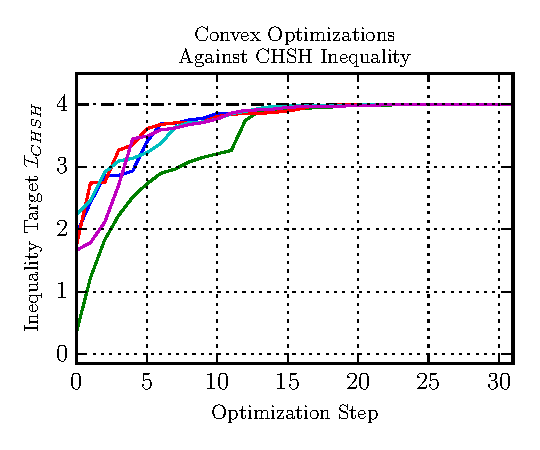
\includegraphics{../../figures/CHSH_convex.pdf}
            \caption{Convex optimizations against $I\tsb{CHSH}$ recover algebraic violation of $4$.}
            \label{fig:CHSH_convex}
        \end{minipage}\hspace{0.04\textwidth}%
        \begin{minipage}[b]{.48\textwidth}
            \centering
            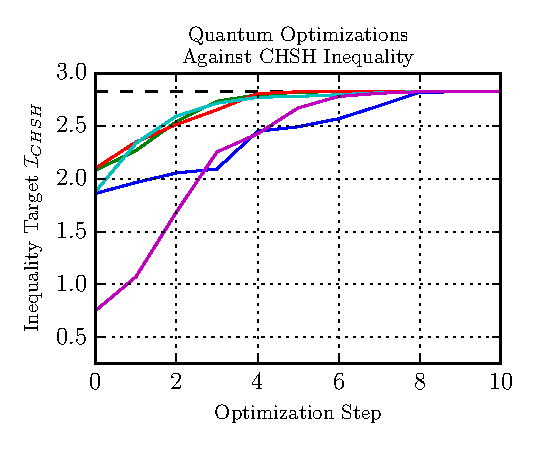
\includegraphics{../../figures/CHSH_quantum.pdf}
            \caption{Quantum optimizations against $I\tsb{CHSH}$ recover maximum violation of $2\sqrt{2}$.}
            \label{fig:CHSH_quantum}
        \end{minipage}
    \end{center}
    \end{figure}

    \todo[TC]{Demonstrate Quantum, Convexity}
    \todo[TC]{Why Inequalities are great for optimizations}
    \todo[TC]{Non-linearity}
    \todo[TC]{Techniques Used}
    \todo[TC]{Finding maximum violation of CHSH easily}
    \todo[TC]{Unreliance when number of parameters increases}
    \todo[TC]{Issues with local minimum}
    \todo[TC]{Using initial conditions close to fritz, obtain greater violation}
    \todo[TC]{Greater violation shares possibilistic structure of fritz and violates CHSH under definition}
    \todo[TC]{Not realizable with maximally entangled qubit states}
    \todo[TC]{Not realizable with separable measurements}
    \todo[TC]{Many non-trivial inequalities to be tested}
    \todo[TC]{inequality -> dist -> inequality evolution}
    \section{Conclusions}
    \todo[TC]{Inflation technique allows one to witness fritz incompatibility}
    \todo[TC]{Linear optimization induces certificates which are incompatibility witnesses}
    \todo[TC]{There are quantum distributions in the Triangle Scenario that are incompatible and different from fritz in terms of entanglement but not possibilistic structure}
    \section{Open Questions \& Future Work}
    The marginal problem has be well studied in various contexts~\cite[\ldots]{Vorobev_1962,Inflation,Fritz_2011}. Reference~\cite{Fritz_2011} contains an excellent summary of its connection to other fields of research including knowledge integration, database theory and coalition games in game theory.
    \todo[TC]{Lots of stuff}
    \appendix
    \section{Common Terminology \& Notation}

    \subsection{Graph Theory}
    \begin{definition}
        \label{def:graph}
        A \term{graph} is an ordered tuple $\br{\nodes, \edges}$ of \textit{nodes} and \textit{edges} respectively where the nodes have the capacity to represent any object while the edges are defined as \textit{pairs} of nodes. Typical, although not necessary, the nodes (edges) are indexed by an index set $\ind_\nodes$ ($\ind_{\edges}$).
        \begin{align*}
            \nodes &= \bc{n_i \mid n_i \in \ind_{\nodes}} \\
            \edges &= \bc{e_i = \bc{n_j, n_k} \mid i \in \ind_{\edges}, j,k \in \ind_{\nodes}}
        \end{align*}
    \end{definition}

    \begin{definition}
        \label{def:directed_graph}
        A \term{directed graph} $\graph$ is a graph where each edge $e$ has an order or \term{direction}.
        \begin{align*}
            \nodes &= \bc{n_i \mid n_i \in \ind_{\nodes}} \\
            \edges &= \bc{e_i = \br{n_j \to n_k} \mid i \in \ind_{\edges}, j,k \in \ind_{\nodes}}
        \end{align*}
    \end{definition}

    \begin{definition}
        \label{def:graph_terms}
        The following definitions are common language in directed graph theory. Let $n, m \in \nodes$ be example nodes of the graph $\graph$.
        \begin{itemize}
            \item The \term{parents of a node}: $\Pa[\graph]{n} \defined \bc{m \mid m \to n}$
            \item The \term{children of a node}: $\Ch[\graph]{n} \defined \bc{m \mid n \to m}$
            \item The \term{ancestry of a node}: $\An[\graph]{n} \defined \bigcup_{i\in\mathbb{W}} \Pa[\graph][i]{n}$ where $\Pa[\graph][i]{n} \defined \Pa[\graph]{\Pa[\graph][i-1]{n}}$ and $\Pa[\graph][0]{n} = n$
        \end{itemize}
        All of these terms can be generalized to sets of nodes $N \subseteq \nodes$ through union over the elements,
        \begin{itemize}
            \item The \term{parents of a node set}: $\Pa[\graph]{N} \defined \bigcup_{n\in N}\Pa[\graph]{n}$
            \item The \term{children of a node set}: $\Ch[\graph]{N} \defined \bigcup_{n\in N}\Ch[\graph]{n}$
            \item The \term{ancestry of a node set}: $\An[\graph]{N} \defined \bigcup_{n\in N}\An[\graph]{n}$
        \end{itemize}
    \end{definition}

    \begin{definition}
        An \term{induced subgraph} of $\graph$ for a subset of nodes $N \subseteq \nodes$ is another graph composed of nodes $N$ and all edges $e$ of the original graph that are contained in $N$.
        \[ \Sub[\graph]{N} \defined \br{N, \bc{e_i \mid i \in \ind_\edges, e_i \subseteq N}} \]
        An \term{ancestral subgraph} of $\graph$ for a subset of nodes $N \subseteq \nodes$ is the induced subgraph due to the ancestry of $N$.
        \[ \AnSub[\graph]{N} \defined \Sub[\graph]{\An[\graph]{N}} \]
    \end{definition}

    \begin{definition}
        \label{def:dag}
        A \term{directed acyclic graph} or \term{DAG} $\graph = \br{\nodes, \edges}$ is an directed graph (see \cref{def:directed_graph}) with the additional property that no node $n$ is in its set of \term{ancestors}.
        \[ \forall n \in \nodes : n \notin \bigcup_{i\in\mathbb{N}} \Pa[\graph][i]{n}\]
        It is critical to note the difference in language between \textit{ancestors} from \textit{ancestry}. The ancestry $\An[\graph]{n}$ of a node $n$ is defined in \cref{def:graph_terms} using \textit{whole} numbers $\mathbb{W}$. In contrast, the ancestors of a node are defined similarly with \textit{natural} numbers $\mathbb{N}$.
    \end{definition}

    \subsection{Probability Theory}

    \begin{definition}
        The \term{product distribution} of two disjoint probability distributions $\prob[V]$ and $\prob[W]$ (where $V \cap W = \emptyset$) is denoted as $\prob[V] \times \prob[W]$.
        \[ \forall f \in \Events{V \cup W} : \br{\prob[V] \times \prob[W]}\br{f} \defined \prob[V][f|_{V}]\tcdot\prob[W][f|_{W}] \]
        A product distribution of $k$ mutually disjoint distributions is defined as,
        \[ \prod_{i\in\bs{k}} \prob[V_i] \defined \br{\prob[V_1] \times \cdots \times \prob[V_k]} \]
    \end{definition}

    \begin{definition}
        The \term{marginalization} of a distribution $\prob[V]$ to a distribution over $W \subseteq V$ is denoted $\sum_{V \setminus W} \prob[V]$ and is defined such that,
        \[ \forall f \in \Events{W} : \br{\sum_{V \setminus W} \prob[V]}\br{f} \defined \sum_{g \in \Ext[V]{f}} \prob[V][g] \]
    \end{definition}

    \section{Exemplary Inequalities}
    \section{Connections to Sheaf-Theoretic Treatment}
    \section{Computationally Efficient Parametrization of the Unitary Group}
    Spengler, Huber and Hiesmayr~\cite{Spengler_2010_Unitary} suggest the parameterization of the unitary group $\mathcal{U}\br{d}$ using a $d\times d$-matrix of real-valued parameters $\lambda_{n, m}$,
    \[ U = \bs{\prod_{m=1}^{d-1} \br{\prod_{n=m+1}^{d} \exp\br{i P_n \lambda_{n,m}}\exp\br{i \si_{m,n} \lambda_{m,n}}}} \tcdot \bs{\prod_{l=1}^{d} \exp\br{iP_l \lambda_{l,l}}}  \eq \label{eq:spengler_unitary} \]
    Where $P_l$ are one-dimensional projective operators,
    \[ P_l = \ket{l}\bra{l} \eq \label{eq:projective_operator} \]
    and the $\si_{m,n}$ are generalized anti-symmetric $\si$-matrices,
    \[ \sigma_{m,n} = -i \ket{m}\bra{n} +i \ket{n}\bra{m} \]
    Where $1 \leq m < n \leq d$. Spengler et. al. proved the validity of \cref{eq:spengler_unitary} in Ref.~\cite{Spengler_2010_Unitary}.

    For the sake of reference, let us label the matrix exponential terms in \cref{eq:spengler_unitary} in a manner that corresponds to their affect on an orthonormal basis $\bc{\ket{1}, \ldots, \ket{d}}$.
    \begin{align}
    \begin{split}
        GP_l &= \exp\br{iP_l \lambda_{l,l}} \\
        RP_{n,m} &= \exp\br{i P_n \lambda_{n,m}} \\
        R_{m,n} &= \exp\br{i \si_{m,n} \lambda_{m,n}}
    \end{split} \eq \label{eq:exp_terms}
    \end{align}
    It is possible to remove the reliance on matrix exponential operations in \cref{eq:spengler_unitary} by utilizing the explicit form of the exponential terms in \cref{eq:exp_terms}. As a first step, recognize the defining property of the projective operators \cref{eq:projective_operator},
    \[ P_l^k = \br{\ket{l}\bra{l}}^k = \ket{l}\bra{l} = P_l \]
    This greatly simplifies the global phase terms $GP_l$,
    \[ GP_l = \exp\br{iP_l \lambda_{l,l}} = \sum_{k=0}^{\inf} \f{\br{iP_l \lambda_{l,l}}^k}{k!} = \mathbb{I} + \sum_{k=1}^{\inf} \f{\br{i \lambda_{l,l}}^k}{k!}P_l^k = \mathbb{I} + P_l \bs{\sum_{k=1}^{\inf} \f{\br{i \lambda_{l,l}}^k}{k!}} = \mathbb{I} + P_l \br{e^{i \lambda_{l,l}} - 1} \eq \label{eq:unitary_GP} \]
    Analogously for the relative phase terms $RP_{n,m}$,
    \[ RP_{n,m} = \cdots = \mathbb{I} + P_n \br{e^{i \lambda_{n,m}} - 1} \eq \label{eq:unitary_RP} \]
    Finally, the rotation terms $R_{m,n}$ can also be simplified by examining powers of $i \sigma_{n,m}$,
    \[ R_{m,n} = \exp\br{i \si_{m,n} \lambda_{m,n}} = \sum_{k=0}^{\inf} \f{\br{\ket{m}\bra{n} - \ket{n}\bra{m}}^k \lambda_{m,n}^k}{k!} \]
    One can verify that the following properties hold,
    \begin{align*}
        \br{\ket{m}\bra{n} - \ket{n}\bra{m}}^0 &= \mathbb{I} \\
        \forall k \in \N, k \neq 0 : \br{\ket{m}\bra{n} - \ket{n}\bra{m}}^{2k} &= \br{-1}^k\br{\ket{m}\bra{m} + \ket{n}\bra{n}} \\
        \forall k \in \N : \br{\ket{m}\bra{n} - \ket{n}\bra{m}}^{2k+1} &= \br{-1}^k\br{\ket{m}\bra{n} - \ket{n}\bra{m}}
    \end{align*}
    Revealing the simplified form of $R_{m,n}$,
    \[ R_{m,n} = \mathbb{I} + \br{\ket{m}\bra{m} + \ket{n}\bra{n}} \sum_{j=1}^{\inf} \br{-1}^j\f{\lambda_{n,m}^{2j}}{\br{2j}!} + \br{\ket{m}\bra{n} - \ket{n}\bra{m}} \sum_{j=0}^{\inf} \br{-1}^j\f{\lambda_{n,m}^{2j+1}}{\br{2j+1}!} \]
    \[ R_{m,n} = \mathbb{I} + \br{\ket{m}\bra{m} + \ket{n}\bra{n}} \br{\cos\lambda_{n,m} - 1} + \br{\ket{m}\bra{n} - \ket{n}\bra{m}} \sin\lambda_{n,m} \eq \label{eq:unitary_R} \]
    By combining the optimizations of \cref{eq:unitary_RP,eq:unitary_R,eq:unitary_GP} together we arrive at an equivalent form for \cref{eq:spengler_unitary} that is computational more efficient.
    \[ U = \bs{\prod_{m=1}^{d-1} \br{\prod_{n=m+1}^{d} RP_{n,m}R_{m,n}}} \tcdot \bs{\prod_{l=1}^{d} GP_l} \eq \label{eq:fast_spengler_unitary} \]
    In quantum mechanics, the global phase of a state $\ket{\psi} \in \Hilb^n$ is a \textit{redundant} parameter. Parameterizing unitaries using \cref{eq:fast_spengler_unitary} is especially attractive since the global phase terms $GP_l$ can be dropped, allowing one to parameterize all unitaries in $\mathcal{U}\br{d}$ up to this degeneracy~\cite{Spengler_2010_Unitary}\footnote{In our implementation, we accomplish this by explicitly setting $\lambda_{l,l} = 0$ in \cref{eq:unitary_GP}}.
    \[ U_{/ GP_l} = \bs{\prod_{m=1}^{d-1} \br{\prod_{n=m+1}^{d} RP_{n,m}R_{m,n}}} \eq \label{eq:fast_spengler_unitary_gp} \]
    \todo[TC]{Explanation of Computational Complexity $\mathcal{O}\br{d^3}$ vs. $\mathcal{O}\br{1}$ using~\cite{Moler_2003}}
    \todo[TC]{Pre-Caching for Fixed dimension $d$}
    \todo[TC]{Talk about inverse via haar measure}

    \section{Parametrization of Quantum States \& Measurements}
    \label{sec:param_quantum_states}
    Throughout \cref{sec:optimizations}, we utilize a variety of parameterizations of quantum states and measurements in order to generate quantum-accessible probability distributions. There are numerous techniques that can used when parameterizing quantum states and measurements~\cite{Petz_2015, Hedemann_2013,Spengler_2010_Unitary,Fujii_2005,James_2001} with applications \todo[TC]{Finish this sentence}. For our purposes, we need to parameterize the space of quantum-accessible distributions $\prob[\mathcal{Q}]$ that are \textit{realized} on the Triangle Scenario. We have implemented $\prob[\mathcal{Q}]$ under the following description.
    \[ \prob[ABC]\br{abc} = \Tr\bs{\netperm^\intercal \rho_{AB}\otimes\rho_{BC}\otimes\rho_{CA} \netperm M_{A,a}\otimes M_{B,b} \otimes M_{C,c}} \eq \label{eq:triangle_quantum_distributions} \]

    \subsection{Quantum States}
    The bipartite states $\br{\rho_{AB}, \rho_{BC}, \rho_{CA}}$ of \cref{eq:triangle_quantum_distributions} were taken to be two-qubit density matrices acting on $\Hilb^2 \otimes \Hilb^2$.\footnote{We also considered qutrit $\Hilb^3$ qutit $\Hilb^4$ states. However for $6$ $d$-dimensional $\Hilb^d$ states, the joint density matrix $\rho$ acts on $\br{\Hilb^d}^{\otimes 6}$ making it a $\br{d^6, d^6}$ matrix with $d^{12}$ entries. Computationally only $d = 2$ was feasible for our optimization tasks.} The space of all such states corresponds to the space of all $4\times 4$ positive semi-definite hermitian matrices with unitary trace. Throughout this section, we refer to these bipartite states simply as $\rho$ unless otherwise indicated. There are three distinct techniques that we have considered.

    Taking inspiration from~\cite{James_2001}, we can parameterize all such density matrices $\rho$ using \term{Cholesky Parametrization}~\cite{Grasmair_2014}. The Cholesky decomposition allows one to write any hermitian positive semi-definite matrix $\rho$ in terms of a lower (or upper) triangular matrix $T$ using $\rho = T^\dagger T$. Our Cholesky parameterization consists of assigning $16$ real-valued parameters $\lambda$ to the entires of $T$ and generating a unitary trace $\rho$ similar to eq. (4.4) of~\cite{James_2001}.
    \[ \rho = \f{T^\dagger T}{\Tr\br{T^\dagger T}} \quad T = \pmtrx{\la_{1}&0&0&0\\\la_{2} + i \la_{3}&\la_{4}&0&0\\\la_{5} + i \la_{6}&\la_{7} + i \la_{8}&\la_{9}&0\\\la_{10} + i \la_{11}&\la_{12} + i \la_{13}&\la_{14} + i \la_{15}&\la_{16}} \eq \label{eq:cholesky_param} \]
    Our deviation from exclusiving using \cref{eq:cholesky_param} is two-fold. First, \cref{eq:cholesky_param} is degenerate in that the normalization indicates only $16 - 1 = 15$ parameters are required for fully generic parameterization of all such states $\rho$. Removing this degeneracy is possible although difficult. Second, the parameters $\lambda_i$ carry no physical meaning associated with the state $\rho$, unlike our next parameterization.

    In Spengler, Huber and Hiesmayr's work~\cite{Spengler_2010_Unitary}, they discuss how to parameterization density matrices $\rho$ acting on $\Hilb^d$ of rank $k$ through it's spectral decomposition,
    \[ \rho = \sum_{i=1}^{k} p_i \ket{\psi_i}\bra{\psi_i} \quad p_i \geq 0, \sum_{i} p_i = 1, k \leq d \eq \label{eq:unitary_param_density} \]
    Where any orthonormal basis $\bc{\ket{\psi_i}}$ of $\Hilb^d$ can be transformed into a computational basis $\bc{\ket{i}}$ by a unitary $U \in \mathcal{U}\br{d}$ such that $\ket{\psi_i} = U\ket{i}$. We refer to \cref{eq:unitary_param_density} as the \term{Spengler Parametrization}. Without loss of generality we parameterize all full-rank ($k=d$) matrices by simultaneously parameterizing the $d=4$ eigenvalues $p_i$ of \cref{eq:unitary_param_density} using \cref{eq:convex_param} and the unitary group $\mathcal{U}\br{4}$ up to global phase equivalence using \cref{eq:fast_spengler_unitary_gp}. Parameterizing $\rho$ using the Spengler parameterization requires $3 + 12 = 15$ parameters; admitting no degeneracies.

    Finally in cases where we wish to restrict ourselves to \textit{pure} bipartite states $\rho = \ket{\psi}\bra{\psi}$, we have the luxury to use a \term{Schmidt Parametrization}. This is accomplished via a Schmidt decomposition $\ket{\psi_{AB}} = \sum_{i}\sigma_i \ket{i_A}\otimes\ket{i_B}$ where normalization demands that $\sum_{i} \sigma_i^2 = 1$, $\bc{\ket{i_A}}$ and $\bc{\ket{i_B}}$ are orthonormal bases for $\Hilb_A$ and $\Hilb_B$ respectively~\cite{Neilsen_Chaung_2011}. Additionally for qubit sources we can \textit{choose} our orthonormal bases to be the computational basis $\bc{\ket{0}, \ket{1}}$ and write,
    \[ \ket{\psi} = \cos^2\br{\lambda_1} \ket{0} \otimes \ket{0} + \sin^2\br{\lambda_1} \ket{1} \otimes \ket{1} \]
    Where only $1$ real-valued parameter $\lambda = \bc{\lambda_1}$ is required to parameterize all pure states up to local unitaries. Pure states are also attractive due to their computational advantage in computing \cref{eq:triangle_quantum_distributions}. If each state $\rho$ is decomposable into $\ket{\psi}\bra{\psi}$, then \cref{eq:triangle_quantum_distributions} can be written as,
    \[ \prob[ABC]\br{abc} = \bramidket{\psi_{AB}\psi_{BC}\psi_{CA}}{\netperm M_{A,a}\otimes M_{B,b} \otimes M_{C,c} \netperm^\intercal}{\psi_{AB}\psi_{BC}\psi_{CA}} \eq \label{eq:pure_state_quantum_triangle} \]
    Avoiding the expensive matrix multiplications of \cref{eq:triangle_quantum_distributions}.
    \subsection{Measurements}
    With full generality, we consider a measurement $M$ to be a \term{projective-operator valued measure (POVM)} represented by a set of hermitian, positive semi-definite operators $\bc{M_i}_{i=1,\ldots,k}$\footnote{The $i$-th element of $M$ is referenced using a subscript $M_i$. The set of measurement elements for a particular party $X$ will be written $M_X$. When both party and element are to be referenced, we write $M_{X,i}$.} acting on $\Hilb^d$ summing to the identity,
    \[ \forall \ket{\phi} \in \Hilb^d : \bra{\phi} M_i \ket{\phi} \geq 0 \quad \sum_{i=1}^{k} M_i = \mathbb{I}_{\Hilb^d} \eq \label{eq:povm} \]
    When considering $k=2$ outcome measurements acting on $\Hilb^4$ we parameterize the first POVM element $M_1$ by using a Cholesky parameterization similar to \cref{eq:cholesky_param} without normalizing for trace. Afterwards, $M_2$ is fully determined by \cref{eq:povm}.
    \[ M_1 = T^\dagger T \quad M_2 = \mathbb{I} - T^\dagger T \eq \label{eq:2_povm}\]
    However, in order for $M_2$ to be positive semi-definite, the largest eigenvalue of $M_1$ has to be less than 1. To see this is a necessary and sufficient constraint, first expand out \cref{eq:2_povm},
    \[ \bramidket{\phi}{M_2}{\phi} = \bramidket{\phi}{\mathbb{I} - M_1}{\phi} = \abs{\phi}^2 - \bra{\phi}\br{\sum_{i=1}^{d}m^{\br{i}}_1 \ket{m^{\br{i}}_1}\bra{m^{\br{i}}_1}}\ket{\phi} \]
    Next write a generic $\ket{\phi} \in \Hilb^d$ in terms of a linear combination of the eigenvectors of $M_1$\footnote{The eigenvectors of $M_1$ form an orthonormal basis for $\Hilb^d$ because $M_1$ is Hermitian}.
    \[ \bramidket{\phi}{M_2}{\phi} = \sum_{j}\abs{\braket{\phi}{m^{\br{j}}_1}}^2 - \sum_{i} m^{\br{i}}_1 \abs{\braket{\phi}{m^{\br{i}}_1}}^2 = \sum_{i} \br{1 - m^{\br{i}}_1} \abs{\braket{\phi}{m^{\br{i}}_1}}^2 \eq \label{eq:eigen_less_one} \]
    Since $\ket{\phi}$ is arbitrary, for each $i$ set $\ket{\phi} = \ket{m^{\br{i}}_1}$ to see that each eigenvalue of $M_1$ needs to be less than $1$.
    \[ \bramidket{m^{\br{i}}_1}{M_2}{m^{\br{i}}_1} = \br{1 - m^{\br{i}}_1} \geq 0 \implies m^{\br{i}}_1 \leq 1 \eq \label{eq:2_povm_suff} \]
    By \cref{eq:eigen_less_one} is not difficult to see that \cref{eq:2_povm_suff} is a sufficient condition. During optimization, \cref{eq:2_povm_suff} can either be enforced passively as a constraint or directly by normalizing $M_1$ by its largest eigenvalue $\max\br{m_1^{\br{i}}}$ whenever necessary.

    When generalizing the above parameterization to more than $2$ outcomes, only necessary conditions were found. Generating $k$-outcome POVM measurements is doable using rejection sampling techniques such as those used in~\cite{Petz_2012} however a valid parameterization with little to no degeneracy was not found. Upon making this observation, a necessary departure to \term{projective-valued measures (PVMs)} is warranted\footnote{Strictly speaking, when the number of outcomes ($k$) \textit{matches} the Hilbert space dimension ($d$), \cref{eq:povm} implies \cref{eq:pvm} by completeness. When considering $4$ outcome measurements on bipartite qubit states in $\Hilb^4$, PVMs are completely general. Moreover, Naimark's dilation theorem guarantees that PVMs acting on $\Hilb^q$ can \textit{emulate} the behaviour of any POVM acting on $\Hilb^d$ provided that $q$ is sufficiently larger than $d$~\cite{Naimark}.}. With loss of generality, consider the set of PVMs $M$ satisfying \cref{eq:povm} in addition to orthogonal and projective properties,
    \[ M_i M_j = \de_{ij} M_i \quad M_i = \ket{m_i}\bra{m_i} \eq \label{eq:pvm}\]
    Parameterizing $M$ for $k$-outcome measurements corresponds to parameterizing the set of all $k$-th order orthonormal sub-bases of $\Hilb^d$.
    First note that any such basis $\bc{\ket{\psi_1}, \ldots, \ket{\psi_k}}$ can be transformed into the computational basis $\bc{\ket{1}, \ldots, \ket{k}}$ by a unitary denoted $U \in \mathcal{U}\br{d}$,
    \[ U \ket{\psi_i} = \ket{i} \]
    With this observation we just need to parameterize the set of all unitaries $\mathcal{U}\br{d}$,
    \[ M = \bc{ U\ket{i}\bra{i}U^\dagger }_{i \in 1, \ldots, k} \]
    Specifically, the projective property each $M_i$ means that the global phase of $U$ is completely arbitrary; one only needs to consider parameterizing unitaries up to global phase \cref{eq:fast_spengler_unitary_gp}. This method was inspired by the \textit{measurement seeding} method of P{\'{a}}l and V{\'{e}}rtesi's~\cite{Pal_2010} iterative optimization technique.

    Analogously to \cref{eq:pure_state_quantum_triangle}, projective measurements offer considerable computational advantage as \cref{eq:triangle_quantum_distributions} can be rewritten as,
    \[ \prob[ABC]\br{abc} = \bramidket{m_{A,a}m_{B,b}m_{C,c}}{\netperm^\intercal \rho_{AB}\otimes\rho_{BC}\otimes\rho_{CA} \netperm}{m_{A,a}m_{B,b}m_{C,c}} \eq \label{eq:pure_meas_quantum_triangle} \]

    \subsection{Network Permutation Matrix}
    \begin{figure}
        \centering
        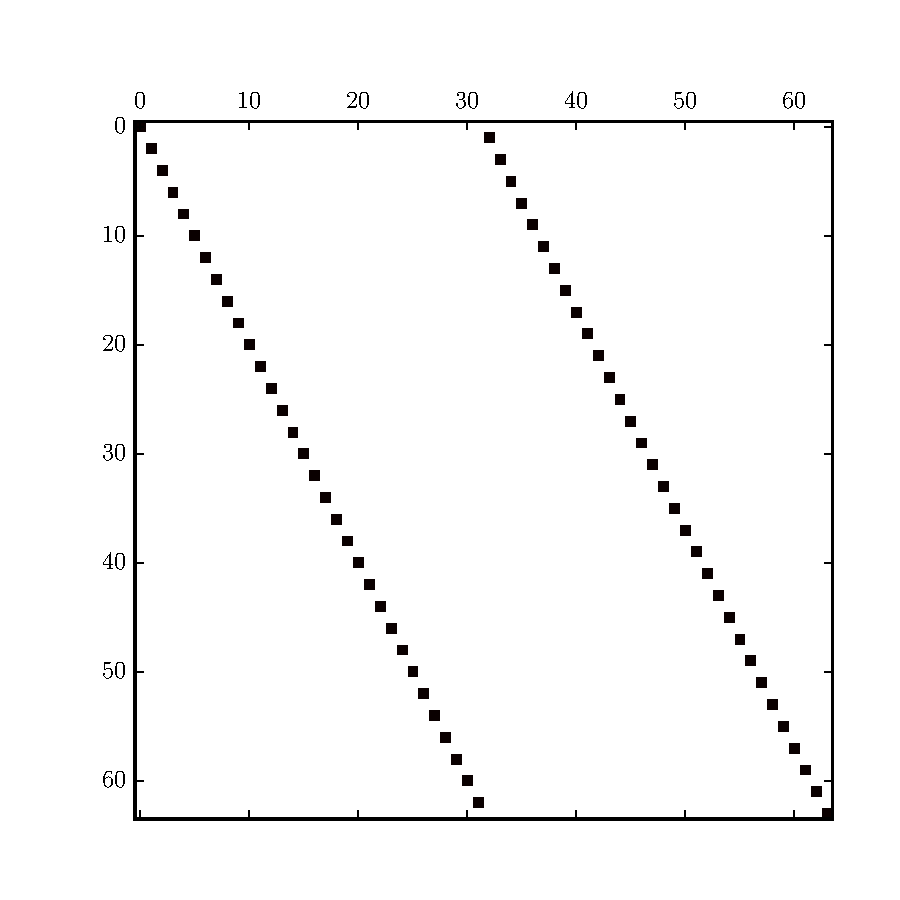
\includegraphics[trim={1cm 1.2cm 1.0cm 1cm},clip,width=0.4\textwidth]{../../figures/perm_mtrx.pdf}
        \caption{The network permutation matrix $\netperm$ for $\br{\Hilb^2}^{\otimes 6}$ realized on the triangle scenario. Black represents a value of $1$ and $0$ otherwise.}
        \label{fig:perm_mtrx}
    \end{figure}
    Finally, we introduce the \term{network permutation matrix} $\netperm$ for the Triangle Scenario of \cref{fig:triangle_scenario}. For bipartite qubit states, $\netperm$ becomes a $64\times64$ bit-wise matrix that acts on the measurements $M$ and is depicted in \cref{fig:perm_mtrx}. To illuminate its necessity, consider \cref{eq:triangle_quantum_distributions} without $\netperm$.
    \begin{align*}
    \prob[ABC]\br{abc} &\stackrel{?}{=} \Tr\bs{\br{\rho_{AB}\otimes\rho_{BC}\otimes\rho_{CA}} \br{M^a_{A}\otimes M^b_{B} \otimes M^c_{C}}}\\
    &= \Tr\bs{\br{\rho_{AB}M^a_{A}}\otimes\br{\rho_{BC}M^b_{B}}\otimes\br{\rho_{CA}M^c_{C}}}\\
    &= \Tr\br{\rho_{AB}M^a_{A}}\Tr{\br{\rho_{BC}M^b_{B}}}\Tr{\br{\rho_{CA}M^c_{C}}}\\
    &= \prob[A\mid \rho_{AB}]\br{a}\prob[B\mid \rho_{BC}]\br{b}\prob[C\mid \rho_{CA}]\br{c}
    \end{align*}
    On an operational level, this corresponds to $A$ making a measurement on \textit{both} subsystems of $\rho_{AB}$ and \textit{not} on any component of $\rho_{CA}$. This is analogously troubling for $B$ and $C$ as well. The network permutation matrix $\netperm$ corresponds to \textit{aligning} the underlying $6$-qubit joint state $\rho$ with the joint measurement $M$. To understand its effect, consider its effect on $6$-qubit pure state $\ket{q_1} \otimes \cdots \otimes \ket{q_6} = \ket{q_1q_2q_3q_4q_5q_6}$ where $\forall i : \ket{q_i} \in \Hilb^2$.
    \[ \netperm\ket{q_1q_2q_3q_4q_5q_6} = \ket{q_2q_3q_4q_5q_6q_1} \]
    $\netperm$ acts as a \textit{partial transpose} on $\br{\Hilb^2}^{\otimes 6}$ by shifting the underlying tensor structure one subsystem to the ``left''. It is uniquely defined by its action on all $2^6$ orthonormal basis elements of $\br{\Hilb^2}^{\otimes 6}$,
    \[ \netperm \defined \sum_{\ket{q_i} \in \bc{\ket{0}, \ket{1}}}\ket{q_2q_3q_4q_5q_6q_1}\bra{q_1q_2q_3q_4q_5q_6} \]
    \subsection{Degeneracy}
    \todo[TC]{Discuss local unitary degeneracy}
    \section{Convex Parametrization of Finite Probability Distributions}
    As discussed in \cref{sec:optimizations}, there is a need to parameterize the family of all probability distributions $\prob[V]$ over a given set of variables $V = \br{v_1, \ldots, v_{\abs{V}}}$. If the cardinality of $O_{V}$ is finite, then this computationally feasible. The space of probability distributions over $n = \abs{O_{V}}$ distinct outcomes forms a $n-1$ dimensional convex polytope naturally embedded in $\R_{\geq 0}^n$~\cite{Brunner_2013} that is parameterizable by $n-1$ real value parameters; normalization $\sum_{o\bs{V} \in O_V} \prob[V][\outc{V}] = 1$ accounts for the `$-1$'. An example of a non-degenerate parameterization of $\prob[V]$ consists of $n-1$ parameters $\lambda = \br{\lambda_1, \ldots, \lambda_{n-1}}, \lambda_i \in \bs{0, \pi/2}$ which generate the $n$ probability values $p_j$ using hyperspherical coordinates~\cite{Hedemann_2013, Spengler_2010_Unitary},
    \begin{equation}
    \begin{gathered}
        \label{eq:convex_param}
        p_j = \cos^2 \lambda_j \prod_{i=1}^{j-1} \sin^2 \lambda_i \quad \forall j \in 1, \ldots, n - 1 \\
        p_n = \prod_{i=1}^{n-1} \sin^2 \lambda_i
    \end{gathered}
    \end{equation}
    Furthermore due to the periodicity of the parameter space $\lambda$, \cref{eq:convex_param} can be used for either constrained or unconstrained optimization problems. For continuity reasons, unconstrained optimizations are performed whenever possible.

    Although non-degenerate, this parameterization suffers from uniformity; a randomly sampled vector of parameters $\lambda$ \textit{does not} translate to a randomly sampled probability $\prob[V]$. An easy-to-implement, degenerate parameterization of $\prob[V]$ can be constructed by simply beginning with $n$ real parameters $\lambda = \br{\lambda_1, \ldots, \lambda_n}$, then making them positive and normalized by their sum\footnote{Strictly speaking, \cref{eq:uniform_param} \textit{also} suffers from non-uniformity; being biased toward uniform probability distributions $\prob[V]$. \todo[TC]{Discuss rejection sampling simplex algorithms}}.
    \[ p_j = \f{\abs{\lambda_j}}{\sum_{i=1}^{n} \abs{\lambda_i}} \quad \forall j \in 1, \ldots, n \eq \label{eq:uniform_param} \]
    For various convex optimization tasks sensitive to initial conditions outlined \cref{sec:optimizations}, the latter parameterization of \cref{eq:uniform_param} generally performed better than the former \cref{eq:convex_param}.

    \bibliography{../references}
\end{document}